%************************************************
\chapter{ML-SAFT: A machine learning framework for PCP-SAFT parameter prediction}\label{ch:deep_gamma} 
%************************************************

\section{Introduction}
\label{sec:intro}
Fluid-phase thermodynamic predictions are required for a range of fine and bulk chemical applications, yet experimental parameterization of thermodynamic models to predict fluid-phase thermodynamics is often time and labor intensive. This motivates the long-standing research interest in predicting parameters of thermodynamic models directly from molecular structures. In addition to established approaches such as group contribution\cite{Fredenslund1975} and quantum mechanical (QM) simulations \cite{Fingerhut2017,Kaminski2020}, recent work has shown that  machine learning (ML) models can be used for predictive thermodynamics. This includes methods for predicting infinite dilution activity coefficients from molecular structures and closely related  solvation free energies using matrix completion\cite{Jirasek2020} and graph neural networks \cite{Vermeire2021, Felton2022, SanchezMedina2022, Qin2023, Rittig2023}. However, the limitation of these works is their lack of thermodynamic consistency that comes with rigorously derived equations of state or their inability to predict multiple thermodynamic properties. 

To enable general and thermodynamically consistent predictions, one approach is to predict thermodynamic model parameters \cite{Abbasi2020, Matsukawa2021, Madani2021, Abdallahelhadj2022, Winter2022}, which also enables simple use in existing process simulation packages. Given the predicted parameters, the thermodynamic model can in turn be used to predict thermodynamic properties. For instance, Winter et al. \cite{Winter2022} developed a model for predicting the parameters of the NRTL activity coefficient model for a wide range of binary mixtures. In this work, we extend this approach of predicting parameters to an Equation of State (EoS), namely Perturbed Chain Polar Statistical Associating Fluid Theory (PCP-SAFT) \cite{Gross2006}, an established extension of the original PC-SAFT EoS to include polar molecules \cite{Gross2001}. The advantages of PCP-SAFT include its ability to predict mixture properties using parameters regressed on pure component data (though we only explore pure component predictions in this work) and its accurate representation of polar compound properties \cite{Cripwell2017}. 

We introduce ML-SAFT, a framework for creating machine learning models that predict PCP-SAFT parameters, shown conceptually in Figure \ref{fig:ML-SAFT_workflow}. The PCP-SAFT parameters are physically interpretable, but they must be regressed or predicted for each molecule.  To train ML models, we develop, to our knowledge, the largest database (988 molecules) of regressed PCP-SAFT parameters using experimental data. We use a combination of deep learning and heuristics to enable large-scale automated regression of PCP-SAFT parameters. We then carry out an extensive evaluation of several machine learning architectures for predicting these regressed PCP-SAFT parameters.

\begin{figure}
    \centering
    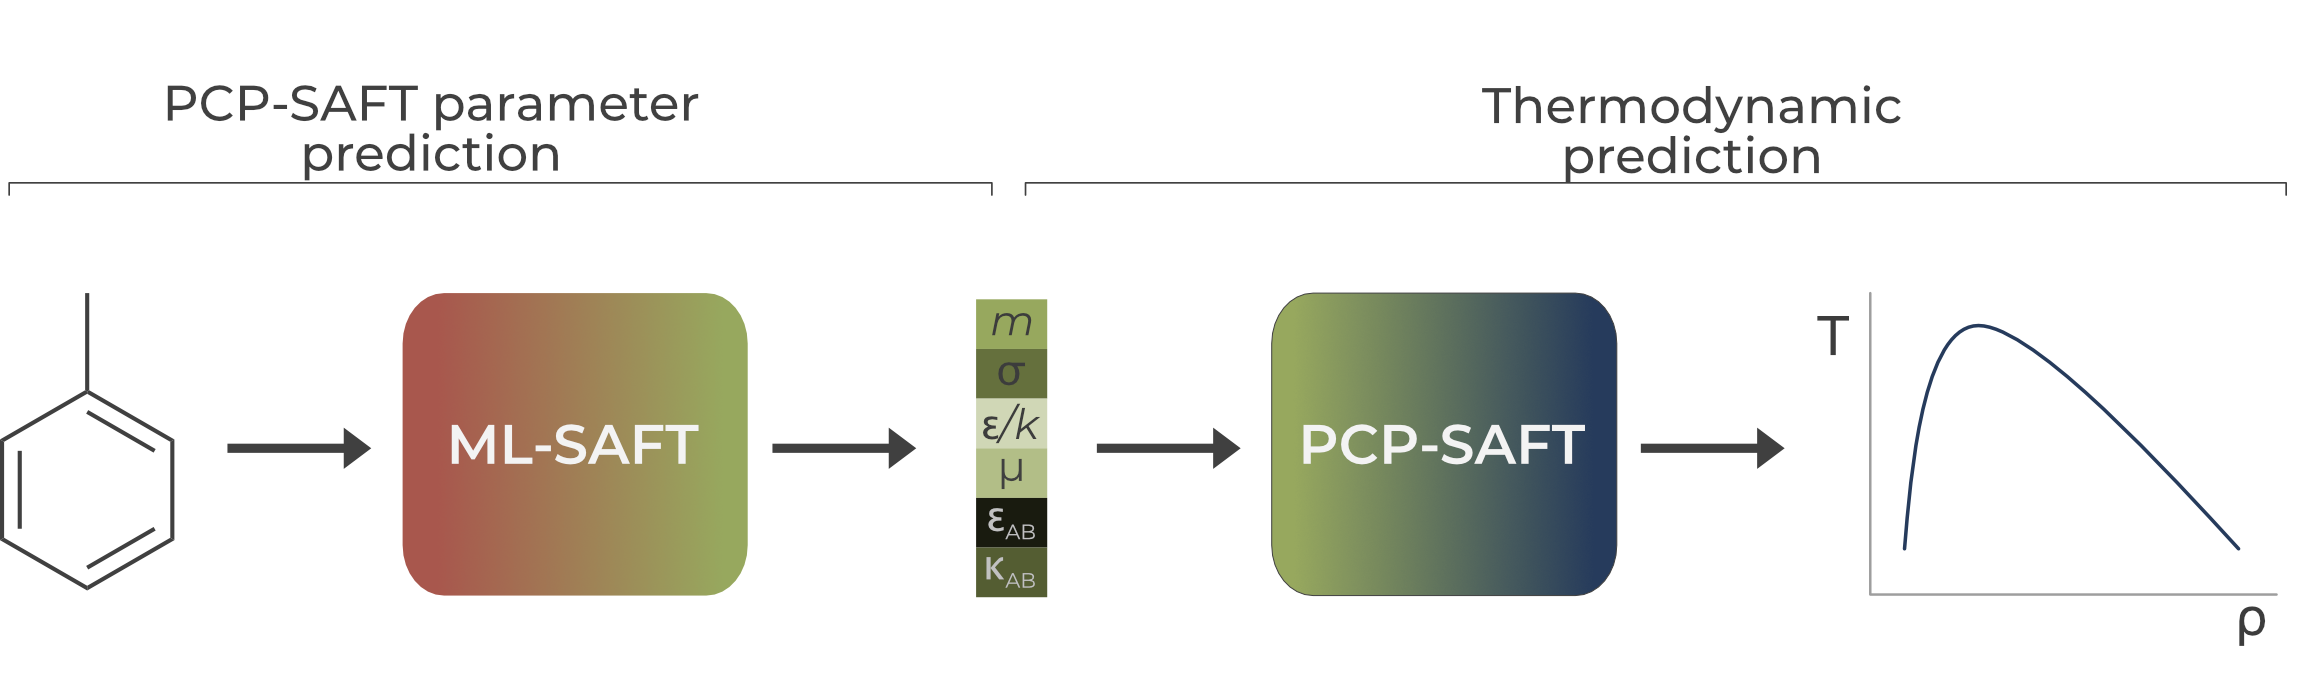
\includegraphics[width=\textwidth]{figures/mlsaft_workflow.png}
    \caption{ML-SAFT is a deep learning model for predicting PCP-SAFT parameters directly from molecular structures. PCP-SAFT parameters predicted by ML-SAFT can be used in any PCP-SAFT implementation. Shown schematically is a density prediction.}
    \label{fig:ML-SAFT_workflow}
\end{figure}

We note that Habicht et al. \cite{Habicht2023} recently developed a feed forward neural network model to predict PC-SAFT parameters from molecular fingerprints. Our framework includes the polar and associating terms and a larger database of regressed PCP-SAFT parameters. We additionally found that random forests outperformed feedforward networks for PCP-SAFT parameter prediction.


he goal of ML-SAFT is to predict the six pure component parameters of PCP-SAFT: $\sigma$, the hard sphere diameter; $m$, number of segments in a chain of a component; $\epsilon/k$, the depth of the well; $\mu$, the dipole moment; and $\epsilon_{AB}$ and $\kappa_{AB}$, the association parameters. We use the implementation of PCP-SAFT in FeO$_{s}$ \cite{Rehner2023}.

\subsection{Baseline predictive PCP-SAFT methods}\label{sec:baselines}

There are several methods in the literature for predicting PCP-SAFT parameters. As comparisons to ML-SAFT, we evaluated two state-of-the-art methods that use QM and a group contribution method respectively.

As a QM method, we applied the Segment-Based Equation of State Parameter Prediction (SEPP) \cite{Kaminski2020}. SEPP obtains $m$, $\sigma$, and $\epsilon/k$ from a multilinear model that uses DFT-calculated features as input, while the dipole moment $\mu$ is obtained directly from QM calculations. An analysis of the surface charge density from COSMO\cite{Klamt1995} was utilized to calculate the associating parameters $\epsilon_{AB}$ and $\kappa_{AB}$. We used the strongest associating site although SEPP can take into account all binary associating interactions. This simplification was made to ensure that the predicted parameters could be used with most PCP-SAFT implementations. Since the multilinear model in SEPP was only fit to alkanes and polar compounds with oxygen and nitrogen, it is not valid for halogens, which are abundant in our dataset.

We used the homosegmented group contribution method from Sauer et al \cite{Sauer2014} as implemented in FeO$_{s}$ \cite{Rehner2023}. For compounds that do not already have groups identified by Sauer et al., we used the group identification from the python package thermo\cite{thermopython} with a modified version of the SMARTS strings from Ruggeri and Takahama (see Supplementary Material) \cite{Ruggeri2016}.

\subsection{Building a dataset for ML-SAFT}\label{subsec:data_set}

To provide data for training ML models, we built, to our knowledge, the largest dataset of PCP-SAFT parameters available to date in the literature (988 molecules).

\subsubsection{Data extraction from the Dortmund Data Bank}

Experimental data were extracted from the 2022 Dortmund Data Bank, which contains data for over 40k unique molecules \cite{dortmunddatabank}. The software package Pura was used to resolve the name or CAS numbers available in the Dortmund database into a cheminformatics friendly identifier, namely SMILES \cite{purapython}. Pura called on PubChem \cite{Kim2020},, the Chemical Identifier Resolver \cite{cir}, OPSIN \cite{Lowe2011}, and the Chemical Abstracts Service\cite{commonchem} to resolve a name or CAS number, and we required that at least two services agreed on the resolved SMILES. Pura resolved 68\% (27.2k/40.3k) of names or CAS numbers to SMILES. 

The experimental data was subsequently filtered to obtain only data that were reasonable for PCP-SAFT regression. Ionic molecules were removed from the dataset as well as any molecules with temperatures outside of the range 200-1000 K and pressures outside the range 10-10000 kPa. Densities greater than 2000 $\text{kg/m}^{3}$ were also excluded. Finally, only molecules with at least four density data points and five vapor pressure data points were considered. After all filtering steps, the experimental data for 988 unique molecules were available for regression of PCP-SAFT parameters. This significant decrease in the size of the data set from 27k to 1k by the filtering step has been noted in other attempts to build models on data available in literature databases \cite{Fitzner2020, Gao2018}. 

\subsubsection{PCP-SAFT parameters regression}

We used the well-established Levenberg-Marquardt (LM) least squares algorithm and experimental vapor pressure and density data, as shown in Figure \ref{fig:ML-SAFT_regression}. The same initial guess shown in Table \ref{tab:regression_params} was applied for all molecules, which was based on the analysis of a large set of PCP-SAFT parameters calculated by QM simulation (see Section \ref{sec:baselines}) \cite{Kaminski2020}. The following equation was applied to calculate the sum of squared errors $\mathcal{L}_i$ for molecule $i$:
\begin{gather}
\begin{aligned}
    \mathcal{L}_i & = \; \sum_j \biggl(\frac{p_{i}^{sat,\text{SAFT}}(T_j) - p_{i}^{sat,\text{EXP}}(T_j)}{ p_{i}^{sat,\text{EXP}}(T_j)}\biggr)^2 \\
    & \; + \sum_j \biggl(\frac{\rho_{i}^{l,\text{SAFT}}(T_j, P_j) - \rho_{i}^{l,\text{EXP}}(T_j, P_j) }{\rho_{i}^{l,\text{EXP}}(T_j, P_j) }\biggr)^2 
\end{aligned}
\end{gather}
where $p_i^{sat}(T_j)$ and $\rho_{i}^{l}(T_j, P_j)$ are the saturation vapor pressure and the liquid density for molecule $i$ respectively at temperature $T_j$ and $P_j$. The superscripts $\text{SAFT}$ and $\text{EXP}$ represent PCP-SAFT predictions and experimental data respectively. 

\begin{table}
    \centering
    \caption{Parameters fitted in PCP-SAFT regression to experimental data.}
    \label{tab:regression_params}
    \begin{tabular}{ccc}
        Parameter name & Bounds & Initial Value \\
        \hline
        $m$ & $1.0 \leq m \leq 10.0$ & 3.26 \\
        $\sigma$ & $2.5 \leq \sigma \leq 5.0$ & 3.69 \\
        $\epsilon/k$ & $100.0 \leq \epsilon/k \leq 1000.0$ & 284 \\
        % $\mu$ & $0.0 \leq \mu \leq 10.0$ & $mu_{pred}$ \\
        $\epsilon_{AB}$ & $0.0 \leq \epsilon_{AB} \leq 4000.0$ & 2400 \\
        $\kappa_{AB}$ & $0.0 \leq \kappa_{AB} \leq 0.01$ & 0.0 \\
    \end{tabular}
\end{table}


\begin{figure}
    \centering
    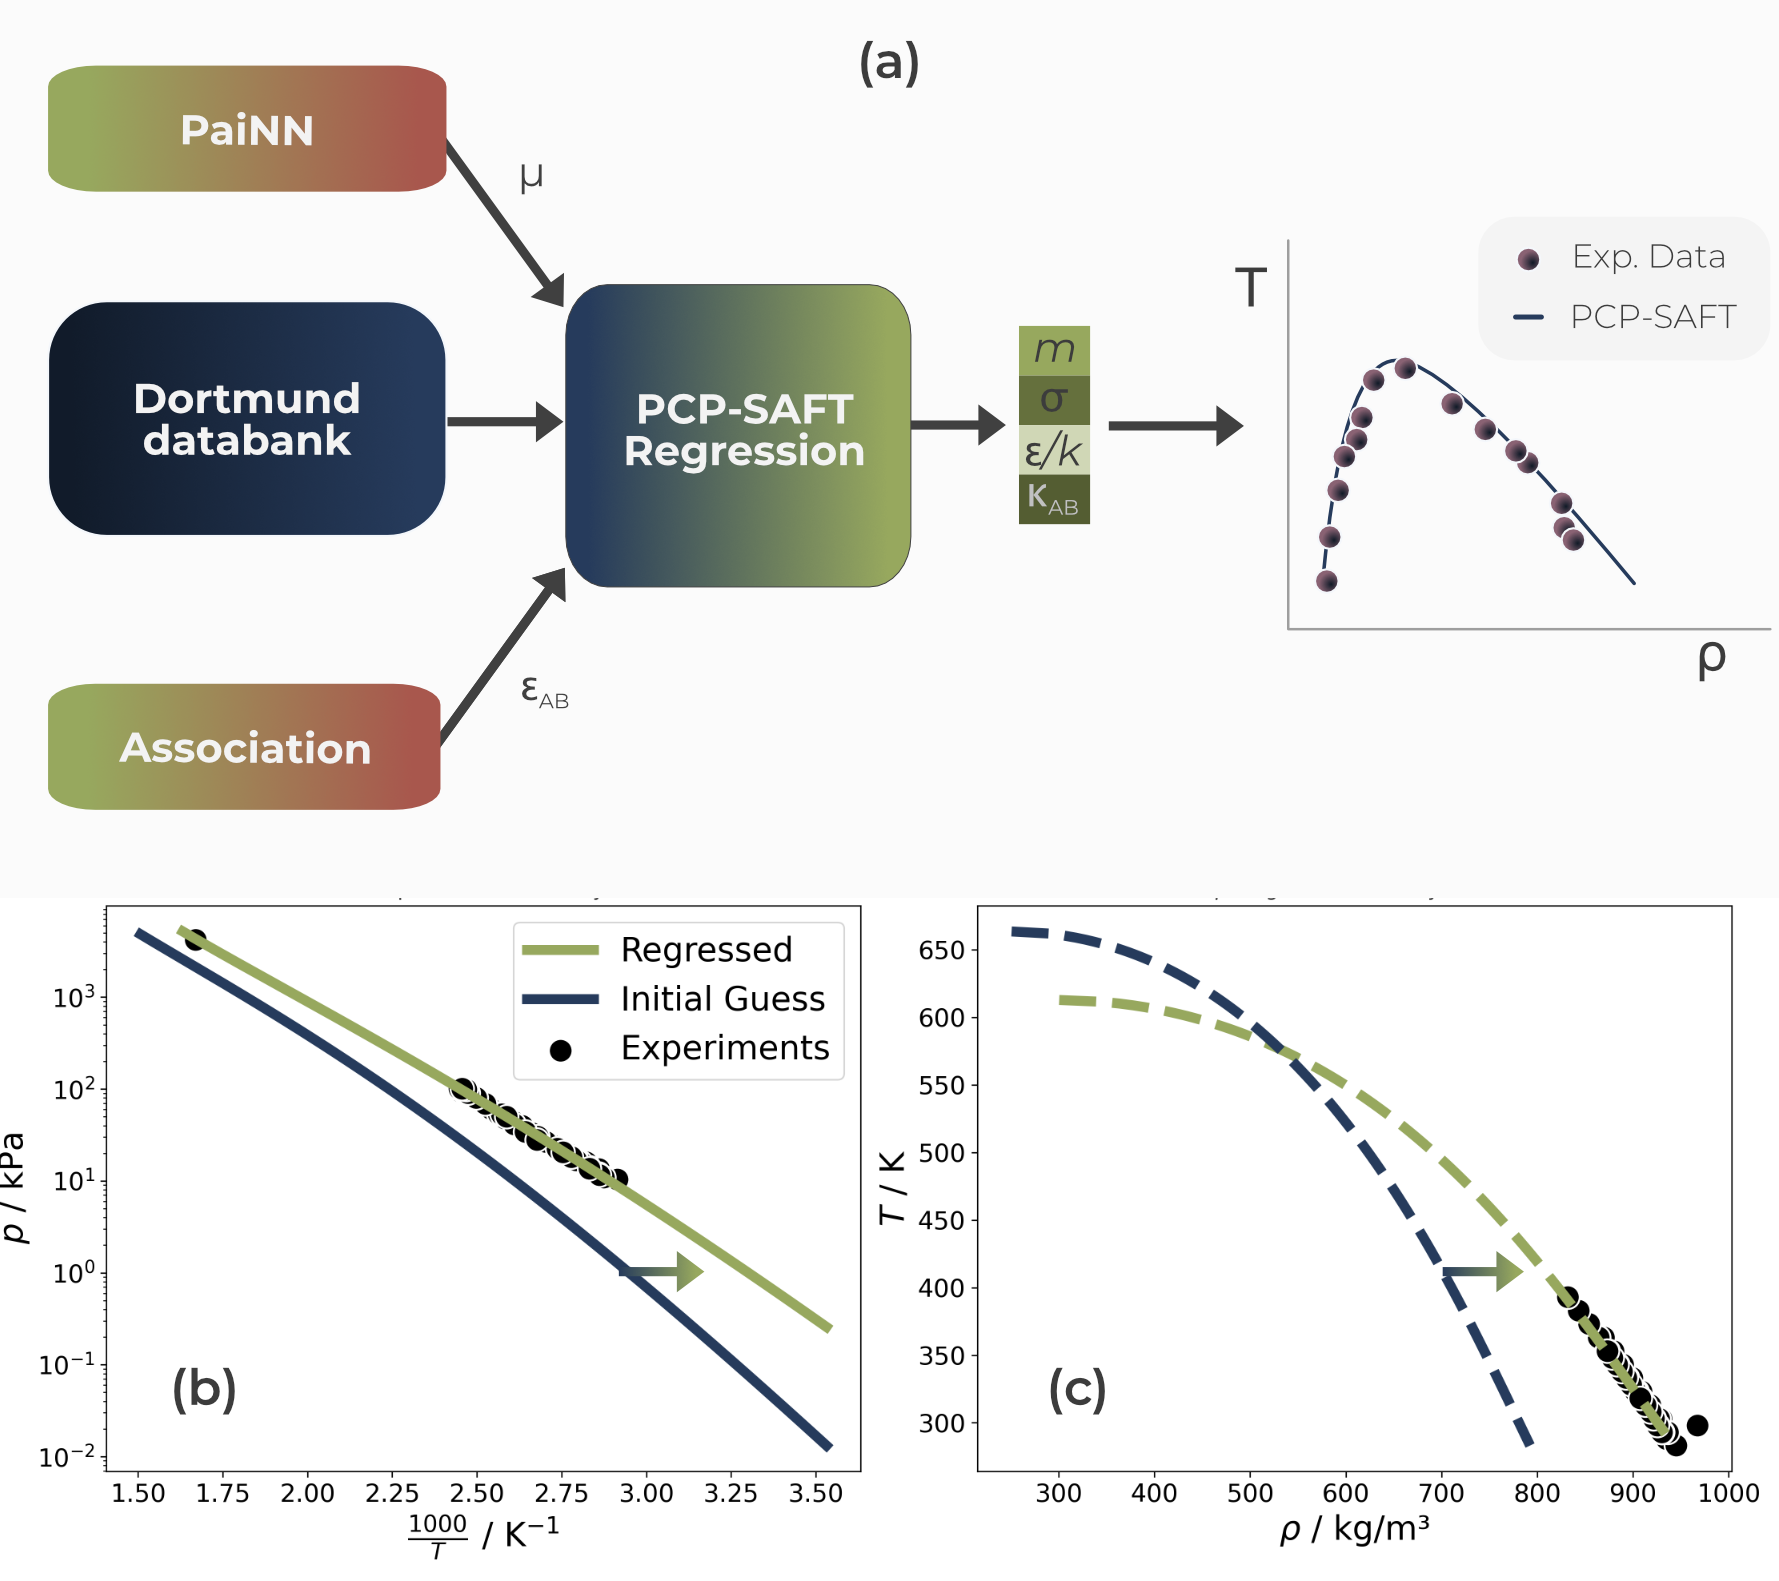
\includegraphics[width=\textwidth]{figures/deepsaft_regression.png}
    \caption{Building a dataset for ML-SAFT: (a) A workflow was developed to automatically regress PCP-SAFT parameters to pure component experimental data. A machine learning model (PaiNN) trained on a combination of DFT and experimental data was used to predict the dipole moments of the experimental dataset, and the other parameters were initialized using standard values. (b-c) Example regression of PCP-SAFT to vapor pressure and density data for 2-ethoxyethanol using the Levenberg-Marquandt algorithm. The dashed line in the density plot represents liquid density.}
    \label{fig:ML-SAFT_regression}
\end{figure}

Only $m$, $\sigma$, $\epsilon/k$ were regressed for all molecules, and $\epsilon_{AB}$ was additionally regressed for associating molecules, while $\mu$ and $\kappa_{AB}$ were not regressed. Instead, we predicted the dipole moment $\mu$ and used heuristics to determine if a molecule was associating (described below). The choice to predict the dipole moment is justified for two reasons. First, dipole moment can usually be measured or calculated on a physical basis, and second, previous work has shown that adjusting the dipole moment causes regression to fail due to high correlation with $\epsilon/k$ \cite{Cripwell2017, deVilliers2011}. 

Therefore, we trained a deep learning model to predict dipole moments using a combination of DFT calculated and experimentally determined dipole moments, as shown in Table \ref{tab:painn_data}. Once trained, the model made dipole moment predictions for hundreds of molecules in seconds. For the model architecture, we chose the tensorial equivariant message passing neural network PaiNN developed by Schütt et al. since it has been shown to give accurate predictions of dipole moment \cite{Schutt2021}. Briefly, PaiNN takes as input a relaxed conformer of a molecule and uses a series of message passing steps on both a vector and rank three tensorial representation to produce a representation of each atom. For training, we used the conformer generation methods shown in Table \ref{tab:painn_data}, and for inference, we used the RDKit ETKDGv3 algorithm to generate conformers \cite{Wang2020}. Subsequently, the dipole moment was calculated using the final vector and tensorial representations of the network:

\begin{equation}
    \vec \mu = \sum_{i=1}^N \vec \mu_{atom}(\vec{\mathbf v_i}) + q_{atom}(\mathbf s_i)\vec r_i
\end{equation}
where $\mathbf s_i$ is the vector representation and $\mathbf v_i$ is the tensorial representation, $\vec r_i$ are the positions of the atoms and $\mu_{atom}$ and $q_{atom}$ are both feedforward networks. Training for 63 epochs resulted in a validation mean absolute error of 0.005 for held-out dipole moment predictions.

We created two heuristics for improving regression of association parameters. First, non-associating molecules were defined as molecules not containing at least one hydrogen-bond acceptor and donor site via RDKit \cite{rdkit}, The associating parameters $\epsilon_{AB}$ and $\kappa_{AB}$ were set to zero for these non-associating molecules. Second, we found that associating parameter $\kappa_{AB}$ could be set to 0.01 and not regressed for all associating molecules while maintaining low regression error. With the deep learning predictions of $\mu$ and the heuristics for association in place, we successfully regressed PCP-SAFT parameters for the 988 available molecules. 

\begin{table}[]
    \centering
    \caption{Data sets used to train PaiNN architecture for predicting dipole moments. $\mu_{source}$ is method used to generate dipole moments; DFT is density functional theory, and Exp. is experimental.}
    \begin{tabular}{ccccc}
         Dataset & $\mu_{source}$ & Conformer Type & Size & Ref.  \\
         \hline
         QM9 & DFT & DFT & 134k & \cite{Ramakrishnan2014}\\
         CRC & Exp. & RDKit\cite{Wang2020} & 482 & \cite{CRC2014} \\
         SEPP & DFT & DFT & 1106 & See Section \ref{sec:baselines}
    \end{tabular}

    \label{tab:painn_data}
\end{table}

\subsubsection{COSMO-RS data generation}

In addition to the Dortmund data bank dataset, we generated a set of PCP-SAFT parameters utilizing pseudo experimental data from the fluid-phase thermodynamics program COSMO-RS.\cite{Klamt2010} Specfically, we generated vapor pressure and density data for 3488 molecules that were already in available 2020 version of the COSMO-RS database. We then regressed PCP-SAFT parameters to these COSMO-RS datasets using the same methods described above. This resulted in 2680 parameters sets available for training.

\subsection{ML-SAFT machine learning models}\label{subsec:ML-SAFT_model}

For prediction of the regressed PCP-SAFT parameters from molecular structures, we tested several machine learning architectures that have previously been successfully applied to molecular property prediction tasks. We included a random forest (RF)\cite{Breiman2001} and a standard feed-forward network (FFN) that use ECFP4 fingerprints as input \cite{Rogers2010}. RFs are known to have strong performance for molecular property prediction in drug discovery but are less common in process systems engineering \cite{Ramsundar2017, Yang2019}. Feed-forward networks were used successfully by Habicht et al. in previous work on predicting PCP-SAFT parameters \cite{Habicht2023}. Furthermore, we developed a standard message passing neural network (MPNN) \cite{Gilmer2017} that has previously been used to predict several thermodynamic parameters including fuel properties\cite{Schweidtmann2020} and activity coefficients \cite{SanchezMedina2022, Rittig2023}. We also tested a variant of an MPNN in which the encoder acts on edges (bonds) instead of nodes (atoms); this architecture is called a directed MPNN (D-MPNN) and has been shown to have state-of-the-art performance for molecular property prediction \cite{Yang2019, Vermeire2021}.

All neural network models (FFN, MPNN and D-MPNN) were trained for 1000 epochs to minimize the mean squared error loss between the predicted and regressed PCP-SAFT parameters using the optimizer Adam\cite{Kingma2015} and the Noam scheduler \cite{Vaswani2017}. The best model checkpoint according to validation loss was used. The learning rate was tuned for each model. We found that using dropout after the pooling step in the MPNN and D-MPNN improved generalization performance. All the final hyperparameters can be found in Table \ref{tab:hyperparameters}.

We experimented with two adaptations of ML to PCP-SAFT prediction. First, since we could already distinguish between associating and non-associating molecules using the heuristic from our regression (i.e., checking the number of association sites), we automatically clamped the association parameters $\epsilon_{AB}$ and $\kappa_{AB}$ to zero for non-associating compounds. We evaluated this clamping of non-associating molecules both as a post-processing step for all models and, for the neural networks, inside the loss function of the neural network. Second, we observed that there were more non-associating than associating molecules in the dataset. Therefore, we tested oversampling of associating molecules in each batch during neural network training using a weighted random sampler:
\begin{equation}
    w_i^{A} = \frac{1}{n_A}
\end{equation}
where $w_i^{A}$ is weight for molecule $i$ with association status $A$ and $n_A$ is the number of molecules of that association status in the whole dataset. We call this oversampling procedure balanced association sampling.

\subsection{Evaluation of predictive PCP-SAFT methods}

To evaluate ML-SAFT models and the baseline predictive PCP-SAFT methods, a set of 81 molecules was held out from training any models and only used for testing. These molecules were selected since the majority could be predicted by SEPP and also had regressed parameters. We then split the remaining 905 molecules into training and validation (5\%) sets using a clustering procedure. Specifically, ECFP fingerprints with 2048 bits were generated using RDKit, and the k-means clustering algorithm\cite{MacQueen1967} was run on five dimensional projections of these fingerprints from UMAP \cite{McInnes2018}. We found three clusters to most effectively model the data, as shown in Figure \ref{fig:splitting}a. Upon manual inspection, we found that the clusters represented chemically interpretable classes of molecules such as alkanes and aromatics. Finally, the molecules were assigned to the training and validation sets so that cluster proportions in each split matched the cluster proportions in the overall dataset using the Stratified Shuffle Split method in scikit-learn \cite{scikit-learn}. This ensured that each split had a balanced set of molecules. As shown in Figure \ref{fig:splitting}c, the functional groups in the train and validation splits were balanced. 

\begin{figure}
    \centering
    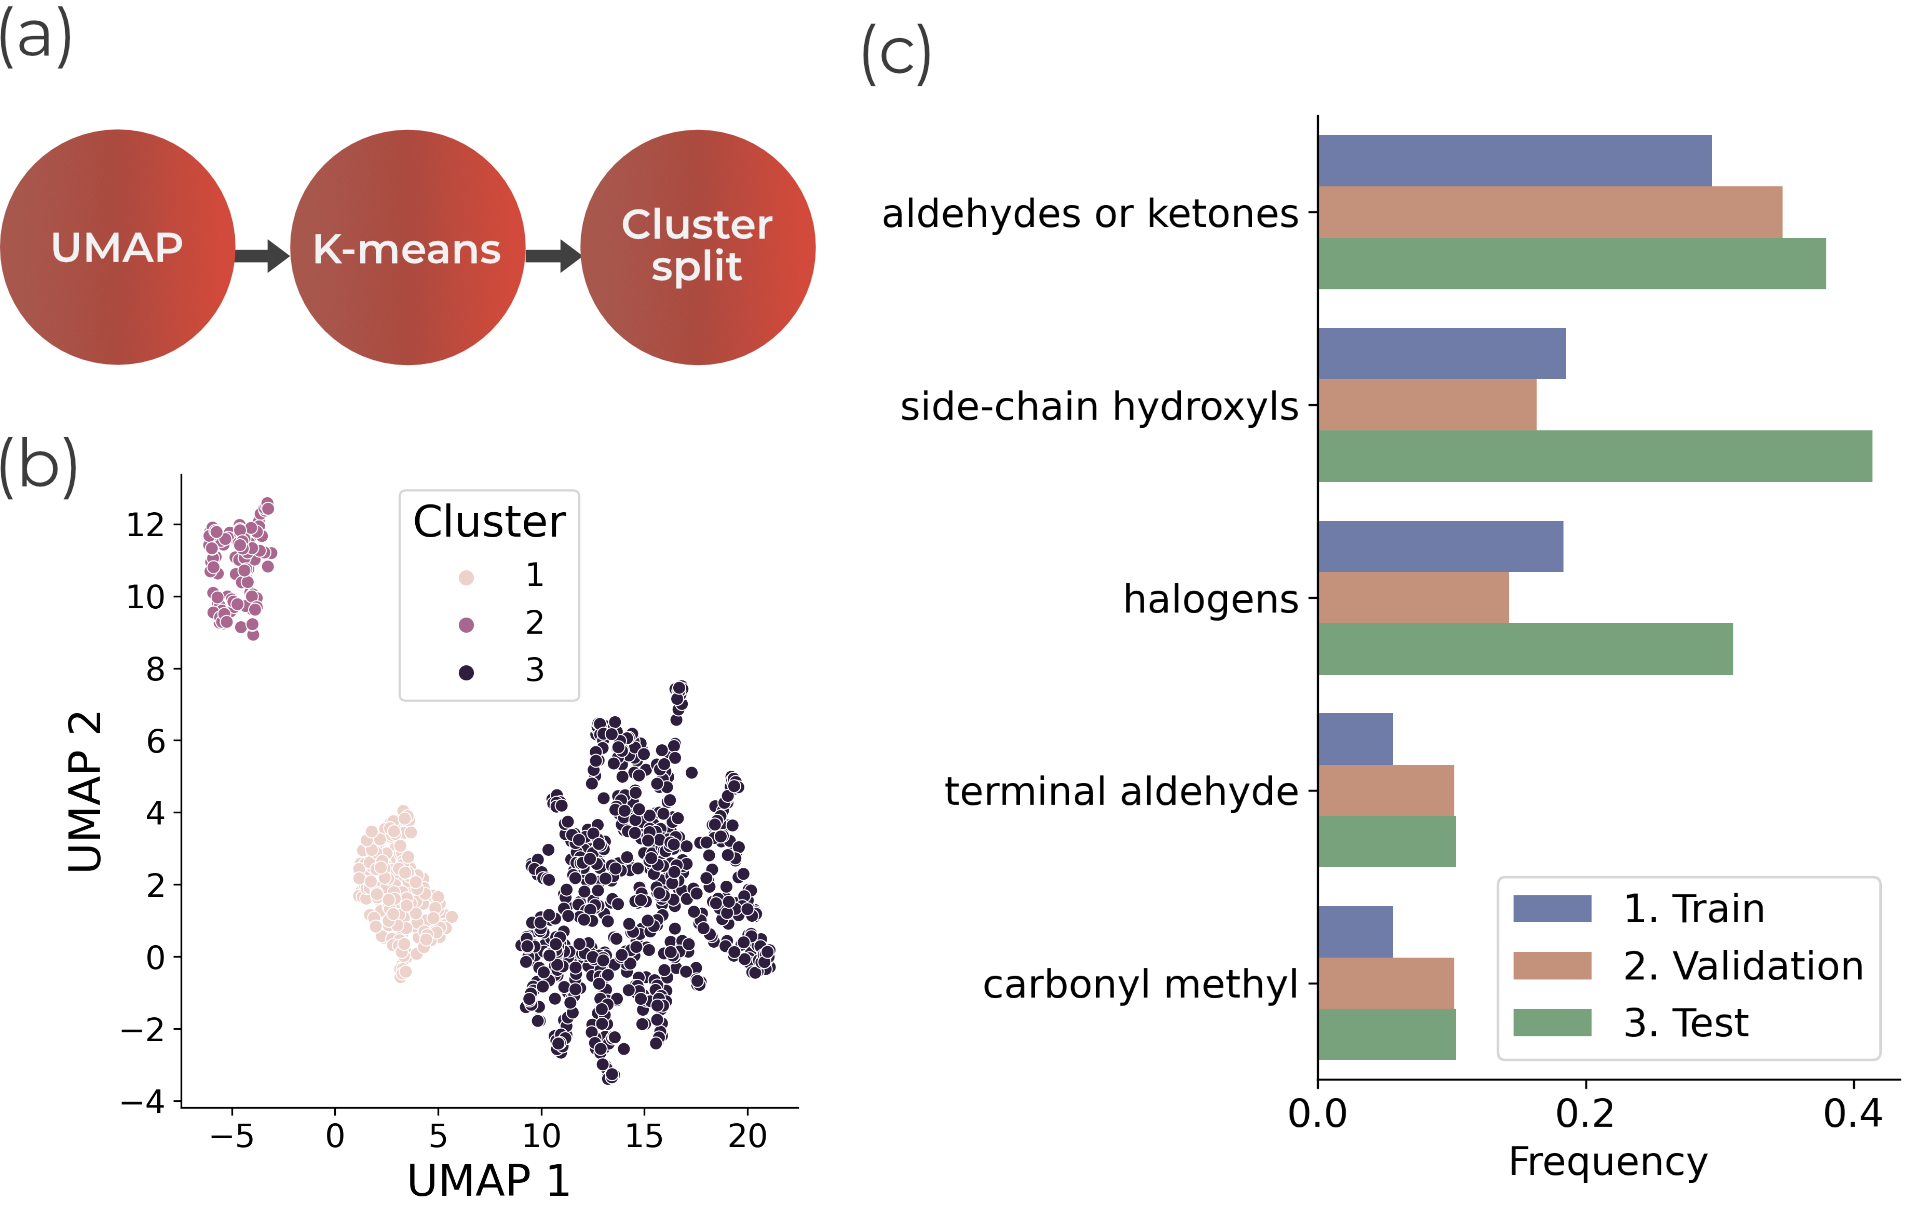
\includegraphics[width=\textwidth]{figures/cluster_split.png}
    \caption{Data splitting for ML-SAFT datasets. (a) Schematic of the workflow for stratified splitting of the ML-SAFT dataset. UMAP\cite{McInnes2018} is used for dimensionality reduction of 2048 bit ECFP fingerprints followed by k-means clustering\cite{MacQueen1967} and cluster splitting using stratified shuffle split in scikit-learn.\cite{scikit-learn} (b) 2D visualization of the clustering using UMAP. (c) The frequency of the top five functional groups in each split are shown. The different functional groups are well balanced between splits.}
    \label{fig:splitting}
\end{figure}

We used two metrics for evaluation of the models. For the evaluation of the error between the parameter predictions and regressed parameters, we applied the root mean squared error (RMSE):
\begin{equation}
    \text{RMSE} = \sqrt{\sum_{i=1}^N \frac{(y_i - \hat y_i)^2}{N}}
\end{equation}
where $y_i$ is the regressed PCP-SAFT parameter and $\hat y_i$ is the predicted PCP-SAFT parameter. For evaluation of the predictions of density and vapor pressure, we used the percent absolute average deviation (\% AAD):
\begin{equation}
    \% AAD = \biggl \vert \sum_j\frac{Q_J - \hat Q_j}{Q_j} \biggr \vert * 100
\end{equation}
where $Q$ is the experimental value of vapor pressure or liquid density and $\hat Q$ is the corresponding PC-SAFT prediction.


\section{Results}

% We first examine the results of the regression of PCP-SAFT parameters and, then, evaluate the effectiveness of different machine learning models in predicting PCP-SAFT parameters. Finally, we compare models trained using the ML-SAFT framework with existing predictive PCP-SAFT methods.

\subsection{A robust regression method for PCP-SAFT parameters}

We sought to develop an automated approach to regressing the PCP-SAFT parameters from experimental data. Since we used the same initial guess for the regression of all 988 molecules in our dataset, we first aimed to understand the quality of this initial guess across the dataset. As shown in Figure \ref{fig:regression_errors}(a-b), the standard initial guess gave liquid density initialization with 35.9\% AAD on average, while the initial accuracy for vapor pressure predictions were significantly worse with an average of 449\% AAD. The larger errors for vapor pressure are likely due to the values for vapor pressure varying over several orders of magnitude. However, after regression, most of the PCP-SAFT predictions using the ML generated PCP-SAFT parameters had less than 5\% AAD, and the overall average was 4.26\% AAD for vapor pressure predictions and 0.62 \% for liquid density predictions, as shown in Figure \ref{fig:regression_errors}(c-d). Empirically, we found that the most important factor for successful regression was the choice of parameter constraints, which we obtained using the maximum and minimum values from all SEPP calculations as an effective solution. 

\begin{figure}
    \centering
    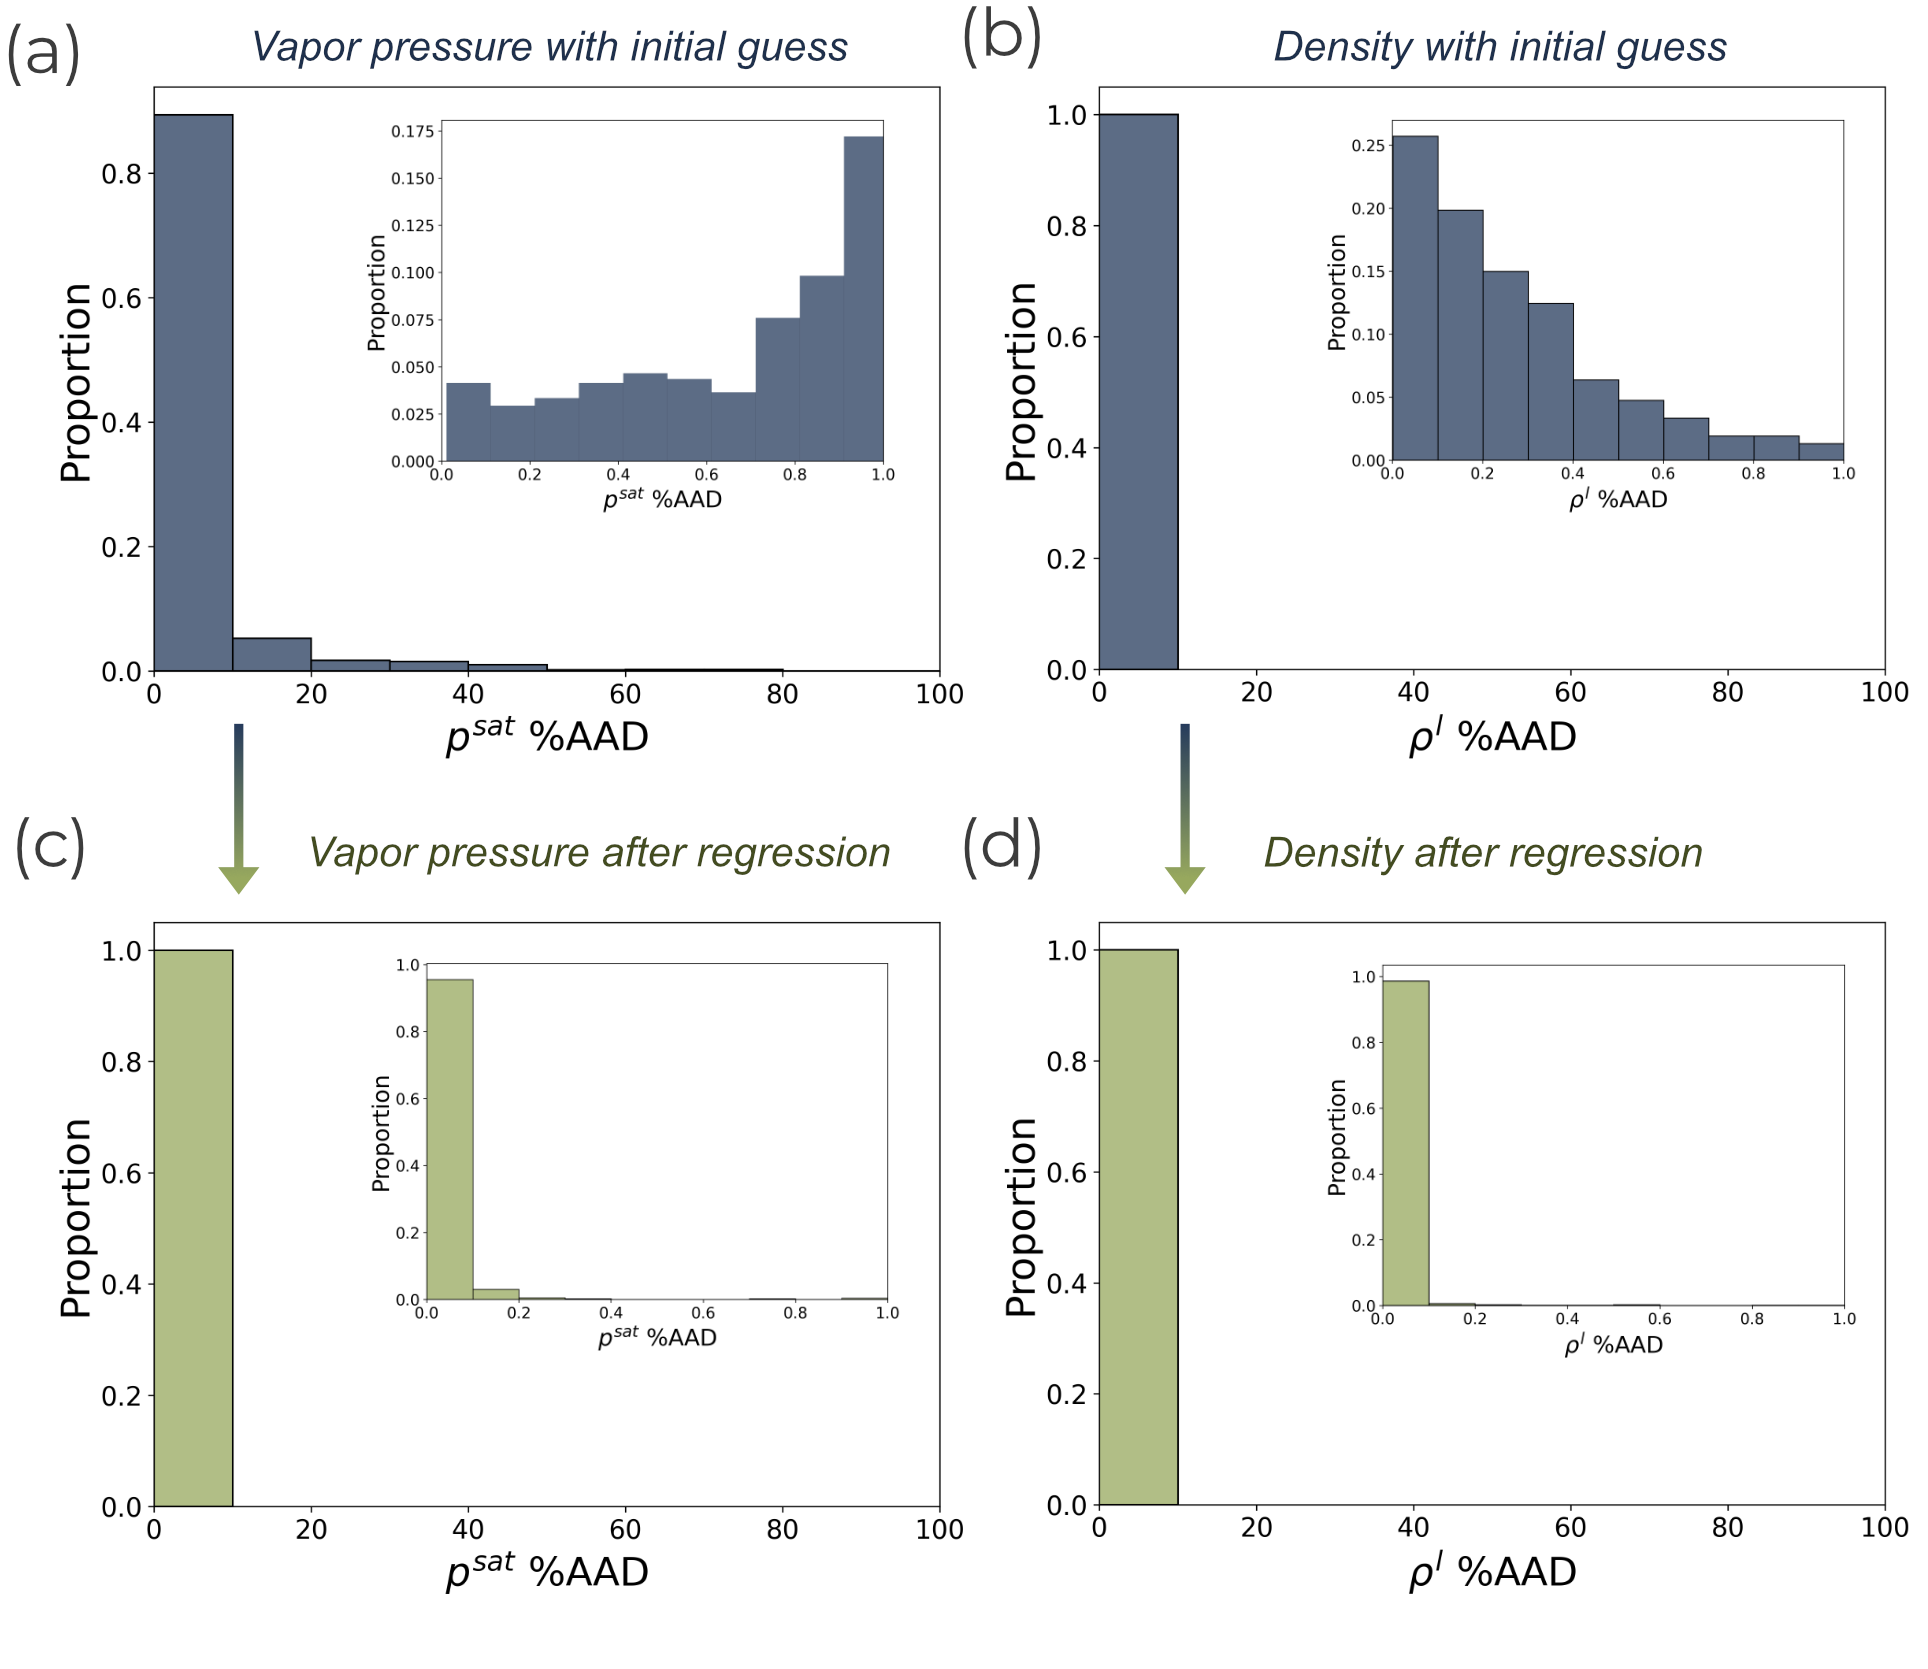
\includegraphics[width=\textwidth]{gfx/Chapter07/regression_errors.png}
    \caption{Distribution of \%AAD  when using PCP-SAFT regressed parameters for all molecules in the ML-SAFT dataset. (a) Initial guess vapor pressure (b) Initial guess liquid density (c) Regressed vapor pressure (d) Regressed liquid density.}
    \label{fig:regression_errors}
\end{figure}

\subsection{ML-SAFT accurately predicts regressed PCP-SAFT parameters}

To evaluate the accuracy of ML models trained to predict the regressed PCP-SAFT parameters, we first compared the PCP-SAFT parameter predictions from the ML models with the regressed PCP-SAFT parameters. Table \ref{tab:parameter_predictions} shows the RMSE of PCP-SAFT parameter predictions from the various machine learning architectures (full parity plots are shown in the \ref{app:parity}). The RF with ECFP fingerprints performed best in predicting all parameters. Even after hyperparameter tuning, all neural network architectures had up to 200\% worse RMSE values. Compared to previous work by Habicht who found that feed forward neural networks gave accurate predictions, our dataset provides a more difficult regression task as we consider a wider range of molecules predict polar parameters for associating molecules; this might explain the lower accuracy of the neural networks in our case. However, the accuracy of predictions of regressed PCP-SAFT parameters might not always translate to the accuracy of thermodynamic predictions, so we also sought to compare the quality of vapor pressure and density predictions.


\begin{table}
	\caption{RMSE (lower is better) of PCP-SAFT parameter predictions compared to regressed PCP-SAFT parameters. The best score for each target is marked in bold. RF: Random forest, FFN: Feed-forward neural network, MPNN: Message-passing neural network, D-MPNN: Directed message-passing neural network.}
        \label{tab:parameter_predictions}
	\begin{center}
		\begin{tabular}{lrrrr}
			 & FFN & D-MPNN & MPNN & RF \\
			\hline
			$m$ & 0.72 & 0.96 & 0.63 & \textbf{0.35} \\
			$\sigma$ & 0.34 & 0.3 & 0.22 & \textbf{0.15} \\
			$\epsilon/k$ & 38 & 27.3 & 25 & \textbf{10.4} \\
			$\epsilon_{AB}$ & 278 & 421 & 325 & \textbf{175} \\
		\end{tabular}
	\end{center}
\end{table}

Table \ref{tab:thermo_parameters} presents the absolute average deviation of PCP-SAFT predictions of vapor pressure and liquid density from experimental data using the predicted PCP-SAFT parameters from various models. The RF model accurately predicted the vapor pressure with an average of 37\% AAD for molecules in the test set. However, the MPNN and D-MPNN performed better on density predictions, despite having less accurate reproduction of the regressed PCP-SAFT parameters. Upon further inspection, we found that this performance difference between the RF and the MPNN family of neural networks was due to the superior performance of the MPNNs on polar compounds such as alcohols. For example, Figure \ref{fig:two_pentanol} shows the vapor pressure and density predictions of PCP-SAFT using the parameter predictions of each ML model. In the case of polar compounds, the RF failed to accurately predict both the vapor pressure and density, while the MPNN and D-MPNN resulted in more accurate predictions for both thermodynamic quantities. We suspect that this difference between the RF and MPNN is due to the enhanced representation capability of the MPNNs.\cite{Gilmer2017, Ramsundar2017}

\begin{table}
	\caption{Comparison of thermodynamic predictions using PCP-SAFT parameters predicted by ML-SAFT models only. The best score for each thermodynamic quantity is
marked in bold. $n$ is the number of molecules in the test set that each method can
predict.}
	\label{tab:thermo_parameters}
	\begin{center}
		\begin{tabular}{lrrrr|r}
			 & FFN & D-MPNN & MPNN & RF & Regressed \\
			\hline
			$n$ & 29 & 29 & 29 & 29 & 29 \\
			\%AAD $p_{sat}$ & 112 & 102 & 62.0 & \textbf{36.2 }& 4.31 \\
			\%AAD $\rho^{L}$ & 22.84 & 8.52 & \textbf{6.56} & 9.92 & 0.45 \\
		\end{tabular}
	\end{center}
\end{table}

We also note that we experimented with several methods to adapt neural network training to PCP-SAFT parameter prediction. In our experiments, we found that there was no significant difference between clamping the values of the association parameters to zero as a post-processing versus during training. Furthermore, balanced association sampling did not offer any noticeable improvement in the accuracy of PCP-SAFT parameter predictions. Although balanced association sampling improved predictions of the association parameter $\epsilon_{AB}$, it degraded the prediction accuracy of the other PCP-SAFT parameters and ultimately led to worse performance on the thermodynamic predictions. Full results of hyperparameter tuning can be found in Table \ref{tab:hyperparameters}.

\begin{figure}
    \centering
    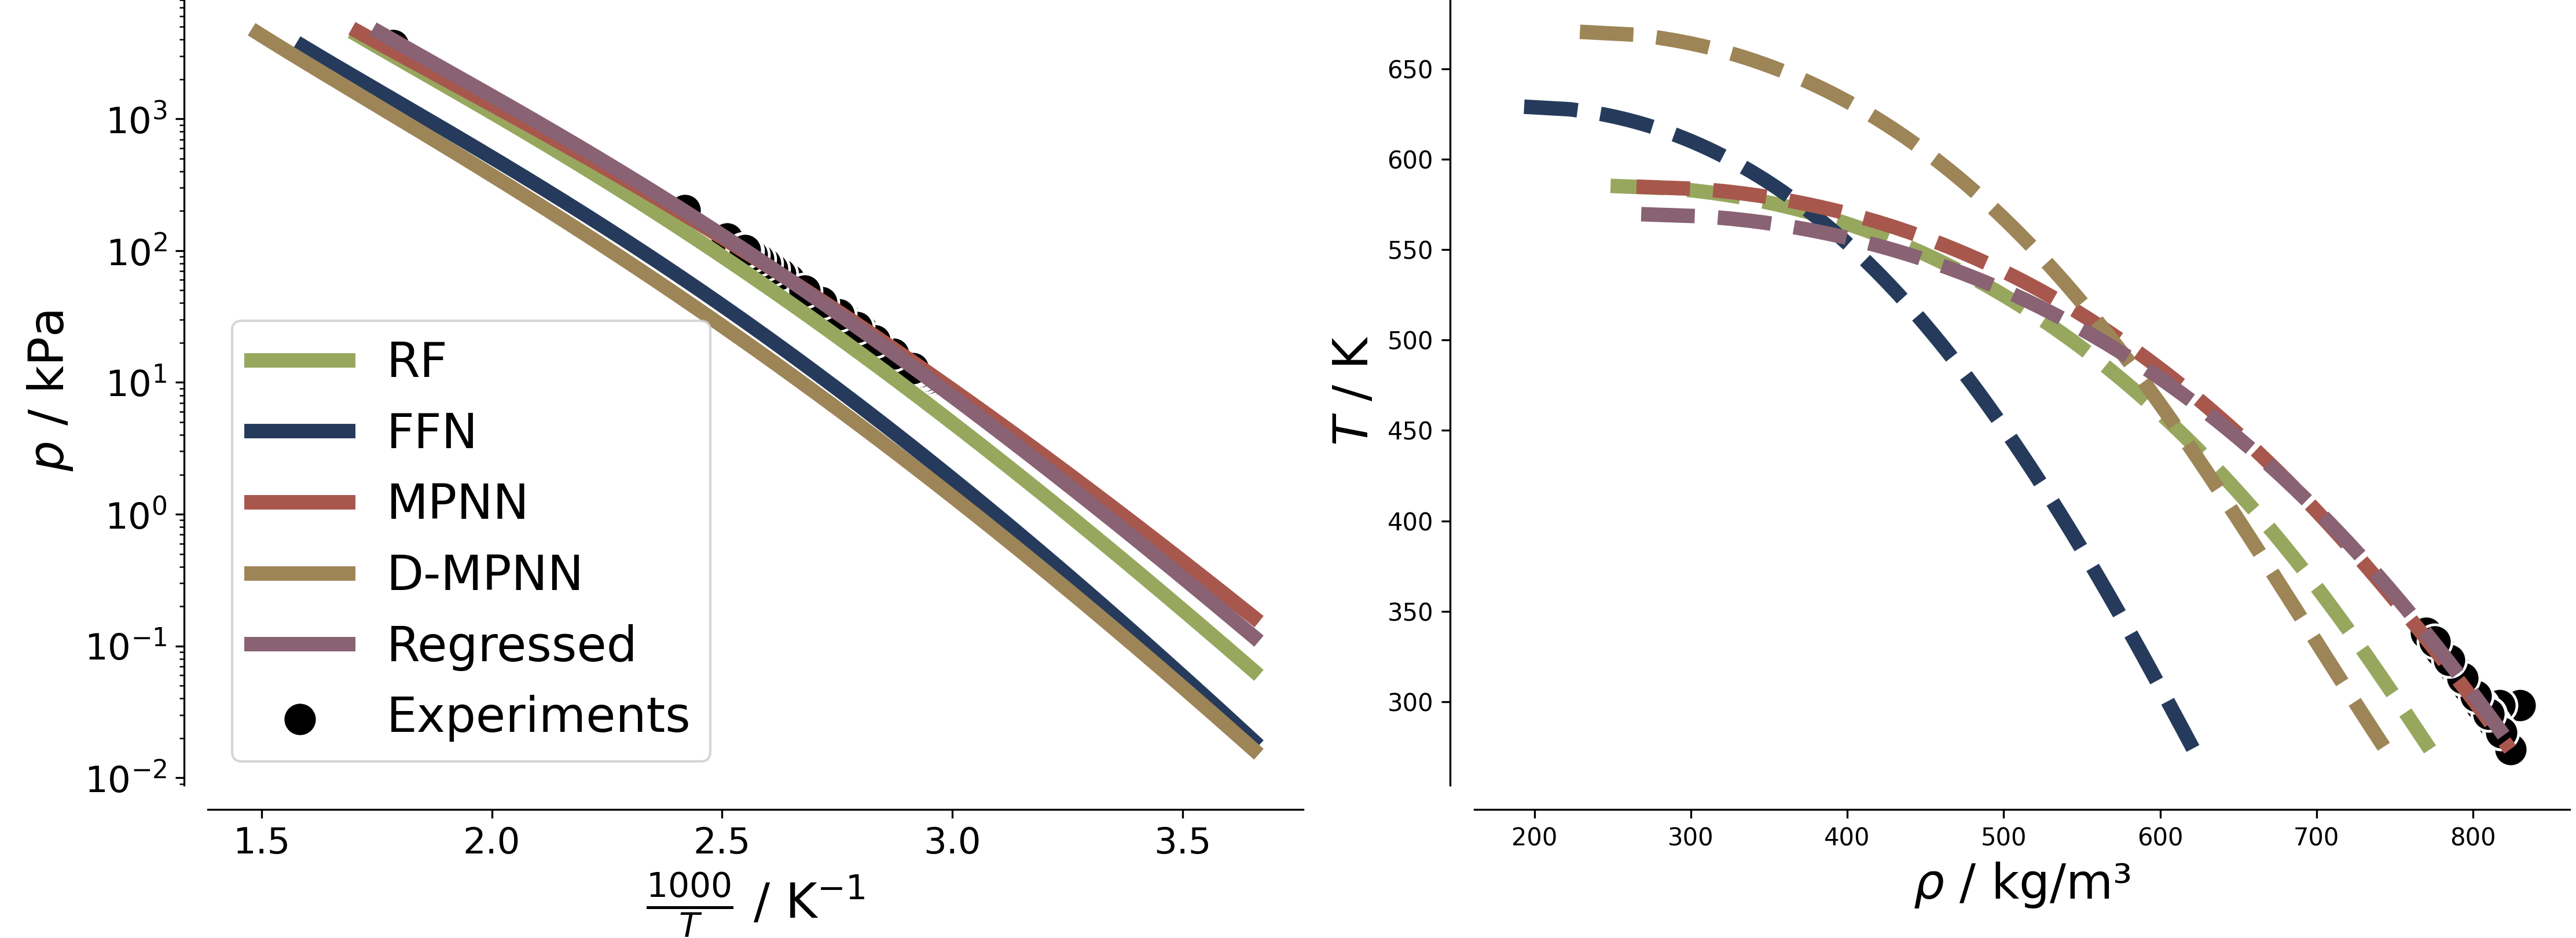
\includegraphics[width=\textwidth]{gfx/Chapter07/2-Pentanol.png}
    \caption{Vapor pressure and density predictions of 2-pentanol of PCP-SAFT using predictions from various machine learning models}
    \label{fig:two_pentanol}
\end{figure}


\subsection{Comparison to existing predictive PCP-SAFT methods}

We compared ML-SAFT to predictions from the QM method SEPP\cite{Kaminski2020} and the group contribution from Sauer et al.\cite{Sauer2014}  Please note that the number of test molecules reduces to 17 as SEPP could not provide predictions to 12 molecules due to its inability to predict halogens. When comparing to SEPP, the RF produces more accurate vapor pressure predictions, while SEPP leads to more accurate density predictions, as shown in Table \ref{tab:sepp}. However, SEPP has a significant associated computational cost that can extend into days, including conformer generation, two DFT calculations, and a COSMO-RS calculation. In contrast, ML-SAFT methods immediately predict the PCP-SAFT parameters from a SMILES string in milliseconds for each molecule while still maintaining a competitive predictive accuracy. 

\begin{table}
	\caption{Comparison of thermodynamic predictions using PCP-SAFT parameters predicted by ML-SAFT models and SEPP.\cite{Kaminski2020} The best score for each thermodynamic quantity is marked in bold. $n$ is the number of molecules in the test set that each method can predict.}
        \label{tab:sepp}
	\begin{center}
		\begin{tabular}{lrrrrr|r}
			 & FFN & D-MPNN & MPNN & RF & SEPP & Regressed \\
			\hline
			$n$ & 17 & 17 & 17 & 17 & 17 & 17 \\
			\%AAD $p_{sat}$ & 90.6 & 54.0 & 71.4 & \textbf{35.1} & 97.9 & 4.52 \\
			\%AAD $\rho^{L}$ & 21.9 & 6.01 & 6.78 & 10.2 & \textbf{2.94} & 0.39 \\
		\end{tabular}

	\end{center}
\end{table}
% Furthermore, we found empirically that our heuristic for identifying associating and non-associating molecules using RDKit\cite{rdkit} worked more effectively than the algorithm based on COSMO charge density used in SEPP.

Comparison with the group contribution method was impaired by the need to convert molecules to groups prior to predictions. Only five of the molecules in our test set had functional groups that were already measured in the database by Sauer et al.\cite{Sauer2014} While the group contribution method performs best for these five molecules (see Table \ref{tab:gc}), the RF predictions are of comparable accuracy. Furthermore, it is difficult to draw conclusions based on such a small subset.

\subsection{Improving MPNN predictions using transfer learning}

We hypothesized that transfer learning could be used to improve the accuracy of the MPNN predictions. As noted in the methods, we used COSMO-RS\cite{Klamt1995, Klamt2010} to generate pseudo experimental data which we the processed through the same regression and training pipeline as the Dortmund data to produce a trained MPNN. We subsequently fixed the message passing encoder of the MPNN and only trained the feedforward readout network; this model we called MPNN-TL. As shown in Figure \ref{fig:cosmo_dortmund}, a subset of the molecules (289) are in both the COSMO-RS and Dortmund databank, and there is good correlation between the PCP-SAFT parameters regressed from tehse datasets. This suggests that the data regressed from  COSMO-RS simulations could be a good pretraining task. 

\begin{figure}
    \centering
    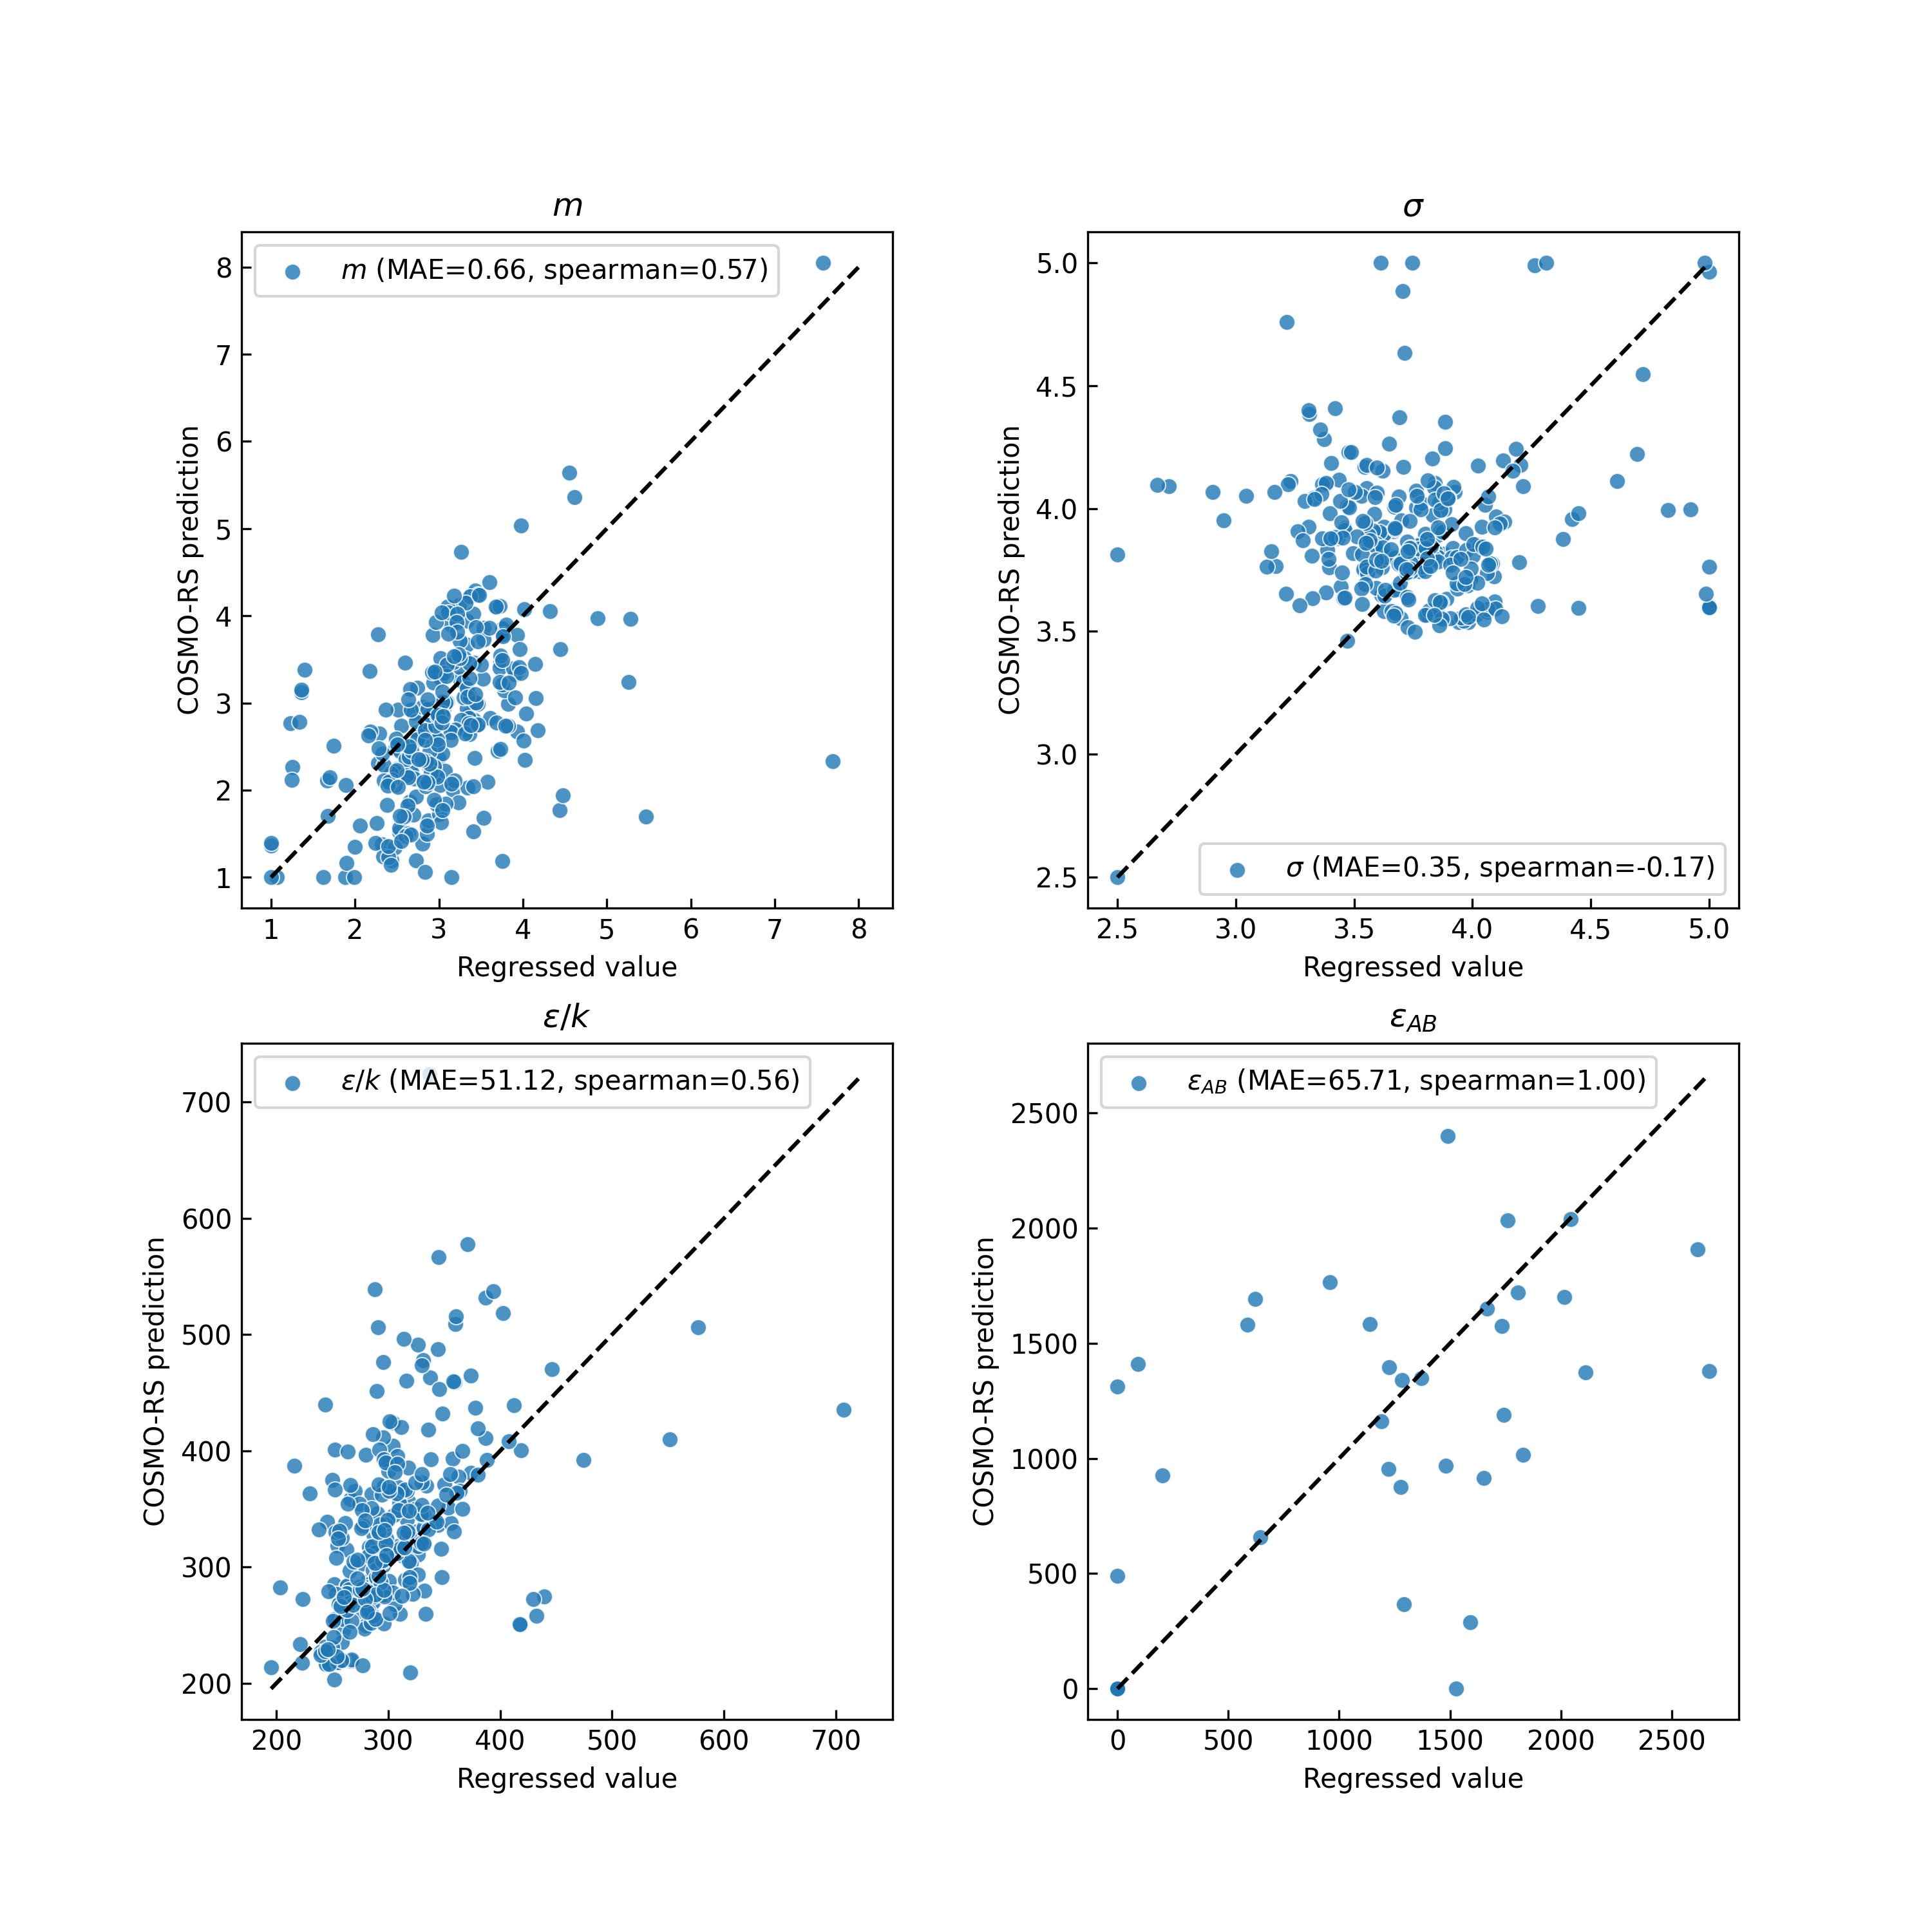
\includegraphics[width=\textwidth]{gfx/Chapter07/cosmo_dortmund_parameter_correlations.png}
    \caption{Parity plots comparing regressed PCP-SAFT parameters based on data from COSMO-RS simulations and the Dortmund databank.}
    \label{fig:cosmo_dortmund}
\end{figure}

The results of the pre-training approach are shown in Table \ref{tab:scores_tl}. On the test set, MPNN-TL outperforms the MPNN giving more accurate predictions of vapor pressure that are on par with the RF. Similarly, the MPNN makes more accurate predictions of density that both the standard MPNN and RF. These results demonstrate that using simulation data can improve the accuracy of neural networks by broadening the scope of moelcular data seen during their training. 

\begin{table}
    \caption{Average absolute deviation percentage of the predictions of vapor pressure and liquid density. The best score for each target is marked in bold.}
    \begin{center}
        \begin{tabular}{lrrr|r}
             & MPNN & MPNN-TL & RF & Regressed \\
            \hline
            $n$ & 29 & 29 & 29 & 29 \\
            \%AAD $p_{sat}$ & 62.08 & 37.88 & \textbf{36.19} & 4.31 \\
            \%AAD $\rho^{L}$ & 6.56 & \textbf{6.41} & 9.92 & 0.45 \\
        \end{tabular}
    \end{center}
    \label{tab:scores_tl}
\end{table}


\section{Discussion}

\begin{table}
	\caption{Comparison of thermodynamic predictions using PCP-SAFT parameters predicted by ML-SAFT models and a group contribution method (GC).\cite{Sauer2014} The best score for each thermodynamic quantity  is marked in bold. $n$ is the number of molecules in the test set that each method can predict.}
    \label{tab:gc}
	\begin{center}
    	\begin{tabular}{lrrrrr|r}
    		 & FFN & D-MPNN & MPNN & RF & GC & Regressed \\
    		\hline
    		$n$ & 5 & 5 & 5 & 5 & 5 & 5 \\
    		\%AAD $p_{sat}$ & 141 & 44.0 & 55.9 & 37.2 & \textbf{27.3} & 3.3 \\
    		\%AAD $\rho^{L}$ & 26.3 & \textbf{3.71} & 8.47 & 11.1 & 5.36 & 0.28 \\
    	\end{tabular}
	\end{center}
\end{table}

In this work, we develop ML-SAFT, a machine learning framework for prediction of PCP-SAFT parameters directly from molecular structures. We developed the largest database of PCP-SAFT parameters (988 molecules) derived from the Dortmund databank. ML-SAFT trained on this dataset accurately predicted the regressed PCP-SAFT parameters, and these predicted PCP-SAFT parameters could be in turn used for accurate predictions of thermodynamic quantities. Random forests had the highest accuracy for the regressed PCP-SAFT parameters and the thermodynamic predictions overall, while the MPNN deep learning architecture was more accurate for polar compounds. 

The best ML-SAFT models (random forests) perform comparably with existing predictive PCP-SAFT methods while being applicable to a wider range of molecules. Group contribution methods require new molecules to be fragmented into groups, and we found that a large fraction of molecules in our dataset were missing parameterized groups or could not be resolved by the automatic fragmentation algorithm. On the other hand, the QM method used for comparison, SEPP, currently is restricted to molecules without halogens as the linear regression model was only fit on alkanes. In contrast, ML-SAFT affords accurate predictions on a wide range of molecules directly from the molecular structures.

There are several ways in which ML-SAFT could be improved. First, the training data for ML-SAFT was primarily small molecules with less than 15 atoms. Previous work has shown that PCP-SAFT can effectively predict properties of larger drug-like molecules (e.g., solubility),\cite{Klajmon2020} and the success of MPNNs in predicting the properties of drug-like molecules suggests that ML-SAFT would be effective given sufficient training data. Second, we do not predict the binary interaction coefficients, which has been shown to significantly improve the quality of PCP-SAFT predictions for mixtures. Future work could address this limitation by training models that contain message-passing between two molecular graphs. This would be a next step towards accurate predictions of multi-component mixture properties using PCP-SAFT.




\section{Author Contributions}

K.C.F developed the concept of ML-SAFT, created the dataset, trained the dipole moment prediction model and all ML-SAFT parameter prediction models and wrote the manuscript. L.R. executed the SEPP calculations, assisted in the PCP-SAFT parameter regression and assisted in manuscript preparation. J.G.R. implemented the MPNN and dipole moment prediction model and assisted in manuscript preparation. K.L., A.M., J.M.-K., C.K, and A.A.L. provided supervision and reviewed the manuscript.


%% The Appendices part is started with the command \appendix;
%% appendix sections are then done as normal sections
\appendix

\section{Analysis of PCP-SAFT parameters}\label{app:sensitivity}

% PCP-SAFT sensitivity analysis was conducted on all molecules in the SEPP dataset  using the Sobol sensitivity analysis method within SALib.\cite{Iwanaga2022} The bounds on each parameter were set to ±10\% of their nominal SEPP values. Figure \ref{fig:sensitivity} shows the results sensitivity analysis.

% Sensitivity analysis shows that $\epsilon/k$ plays a significant role in the prediction of vapor pressure, as well as $\sigma$, $m$, and the association parameters $\epsilon_{AB}$ and $\kappa_{AB}$. However, the vapor pressure predictions are not sensitive to the dipole moment $\mu$, a trend that is also observed for density predictions. For density, $\sigma$ is important while other parameters are less sensitive. 

% \begin{figure}
%     \centering
%     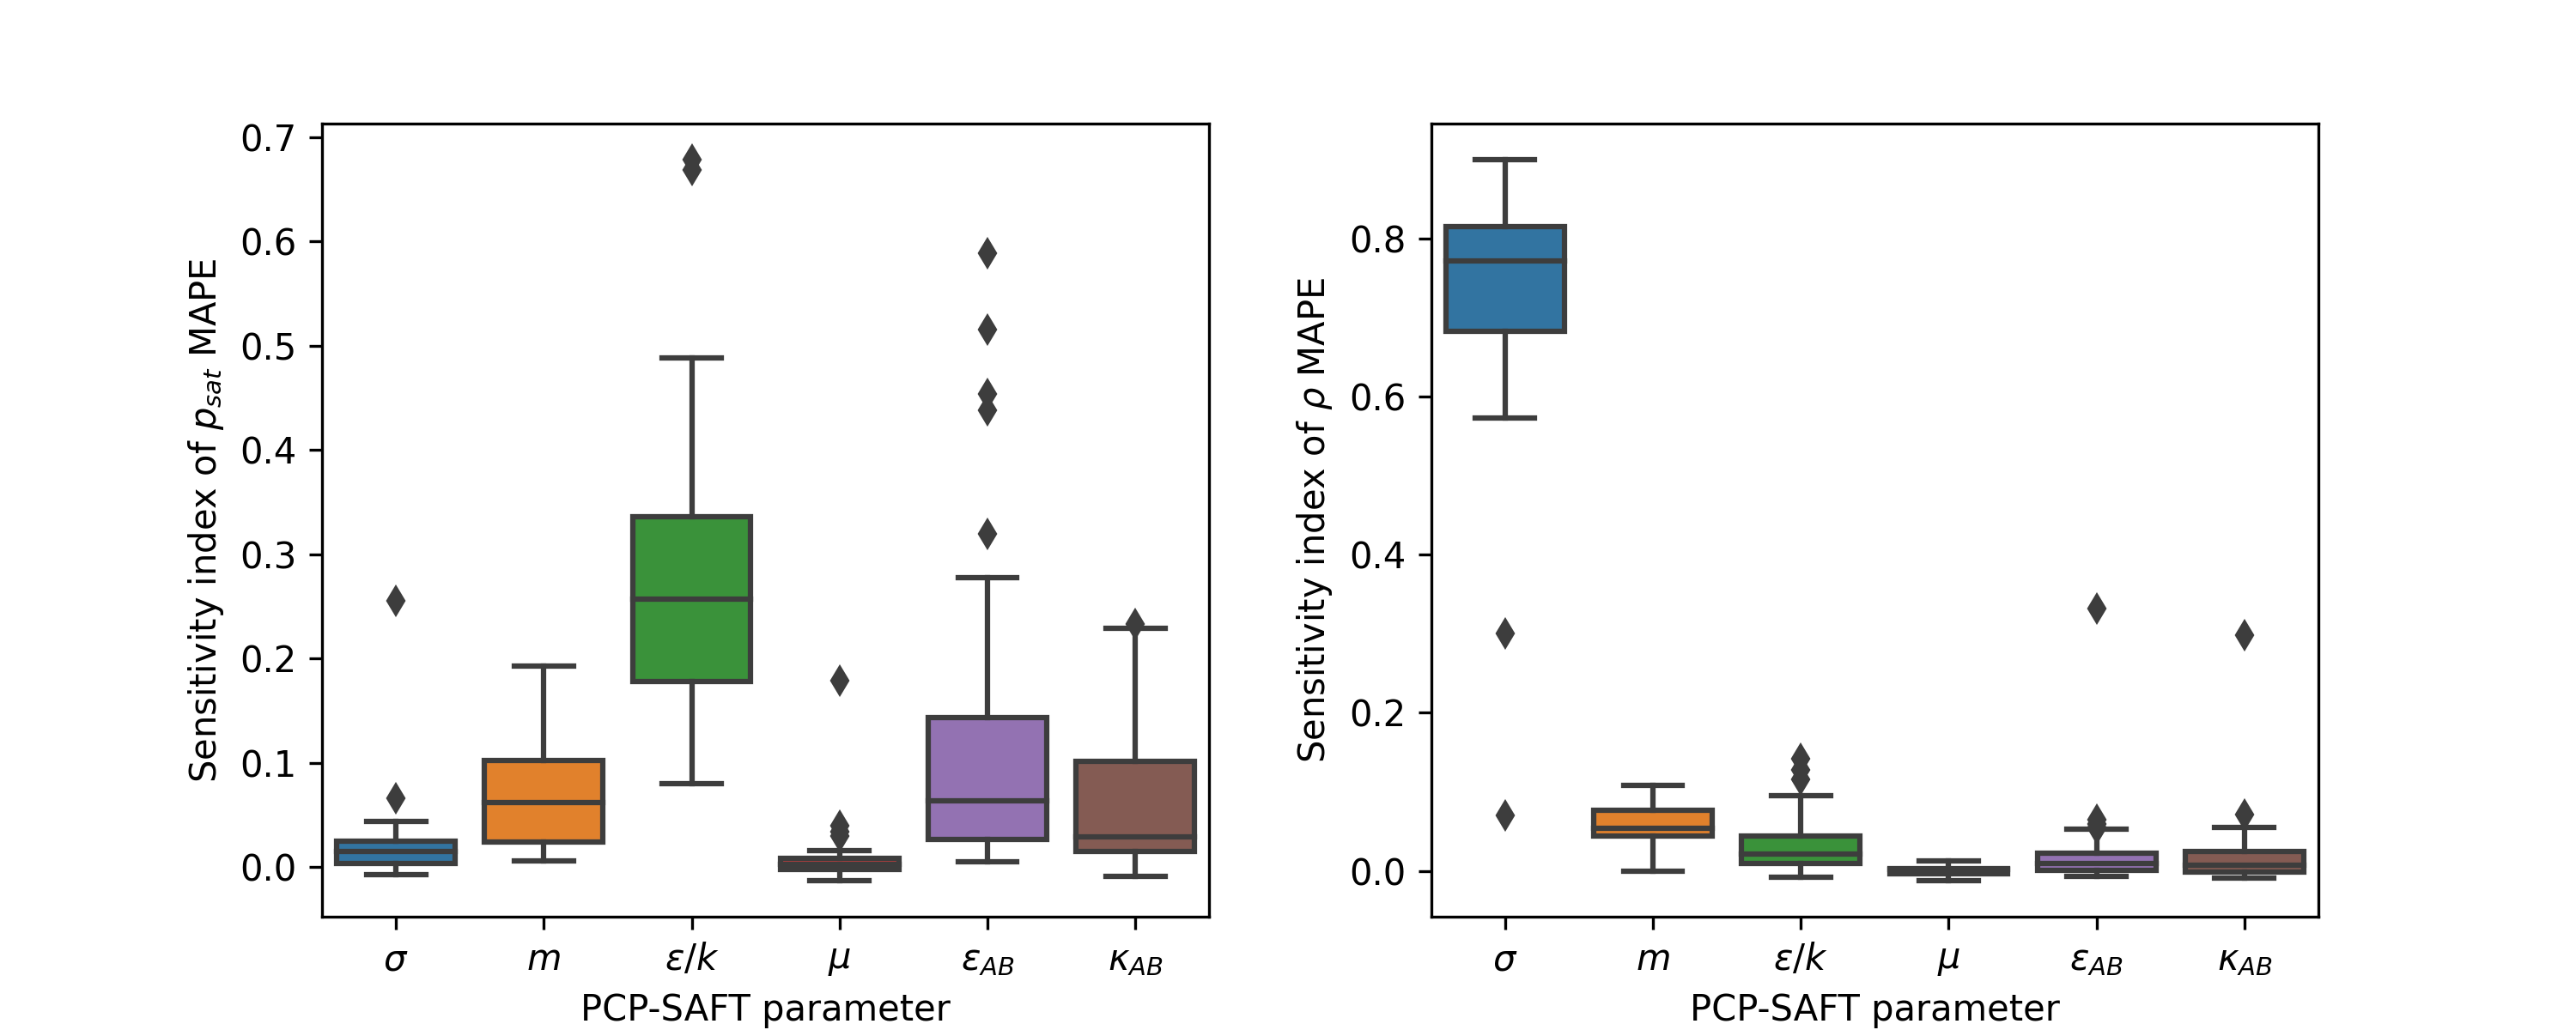
\includegraphics[width=\textwidth]{gfx/Chapter07/sensitivity_analysis_boxplot.png}
%     \caption{Results of sensitivity analysis of PCP-SAFT parameters on vapor pressure and density}
%     \label{fig:sensitivity}
% \end{figure}


Figure \ref{fig:molecular_weight} shows each of the four parameters predicted by ML-SAFT versus the molecular weight of the molecules for the ML-SAFT dataset. We see a positive correlation between molecular weight and $m$ and $\sigma$, while little to no correlation is observed for $\epsilon/k$ and $\epsilon_{AB}$.

\begin{figure}
    \centering
    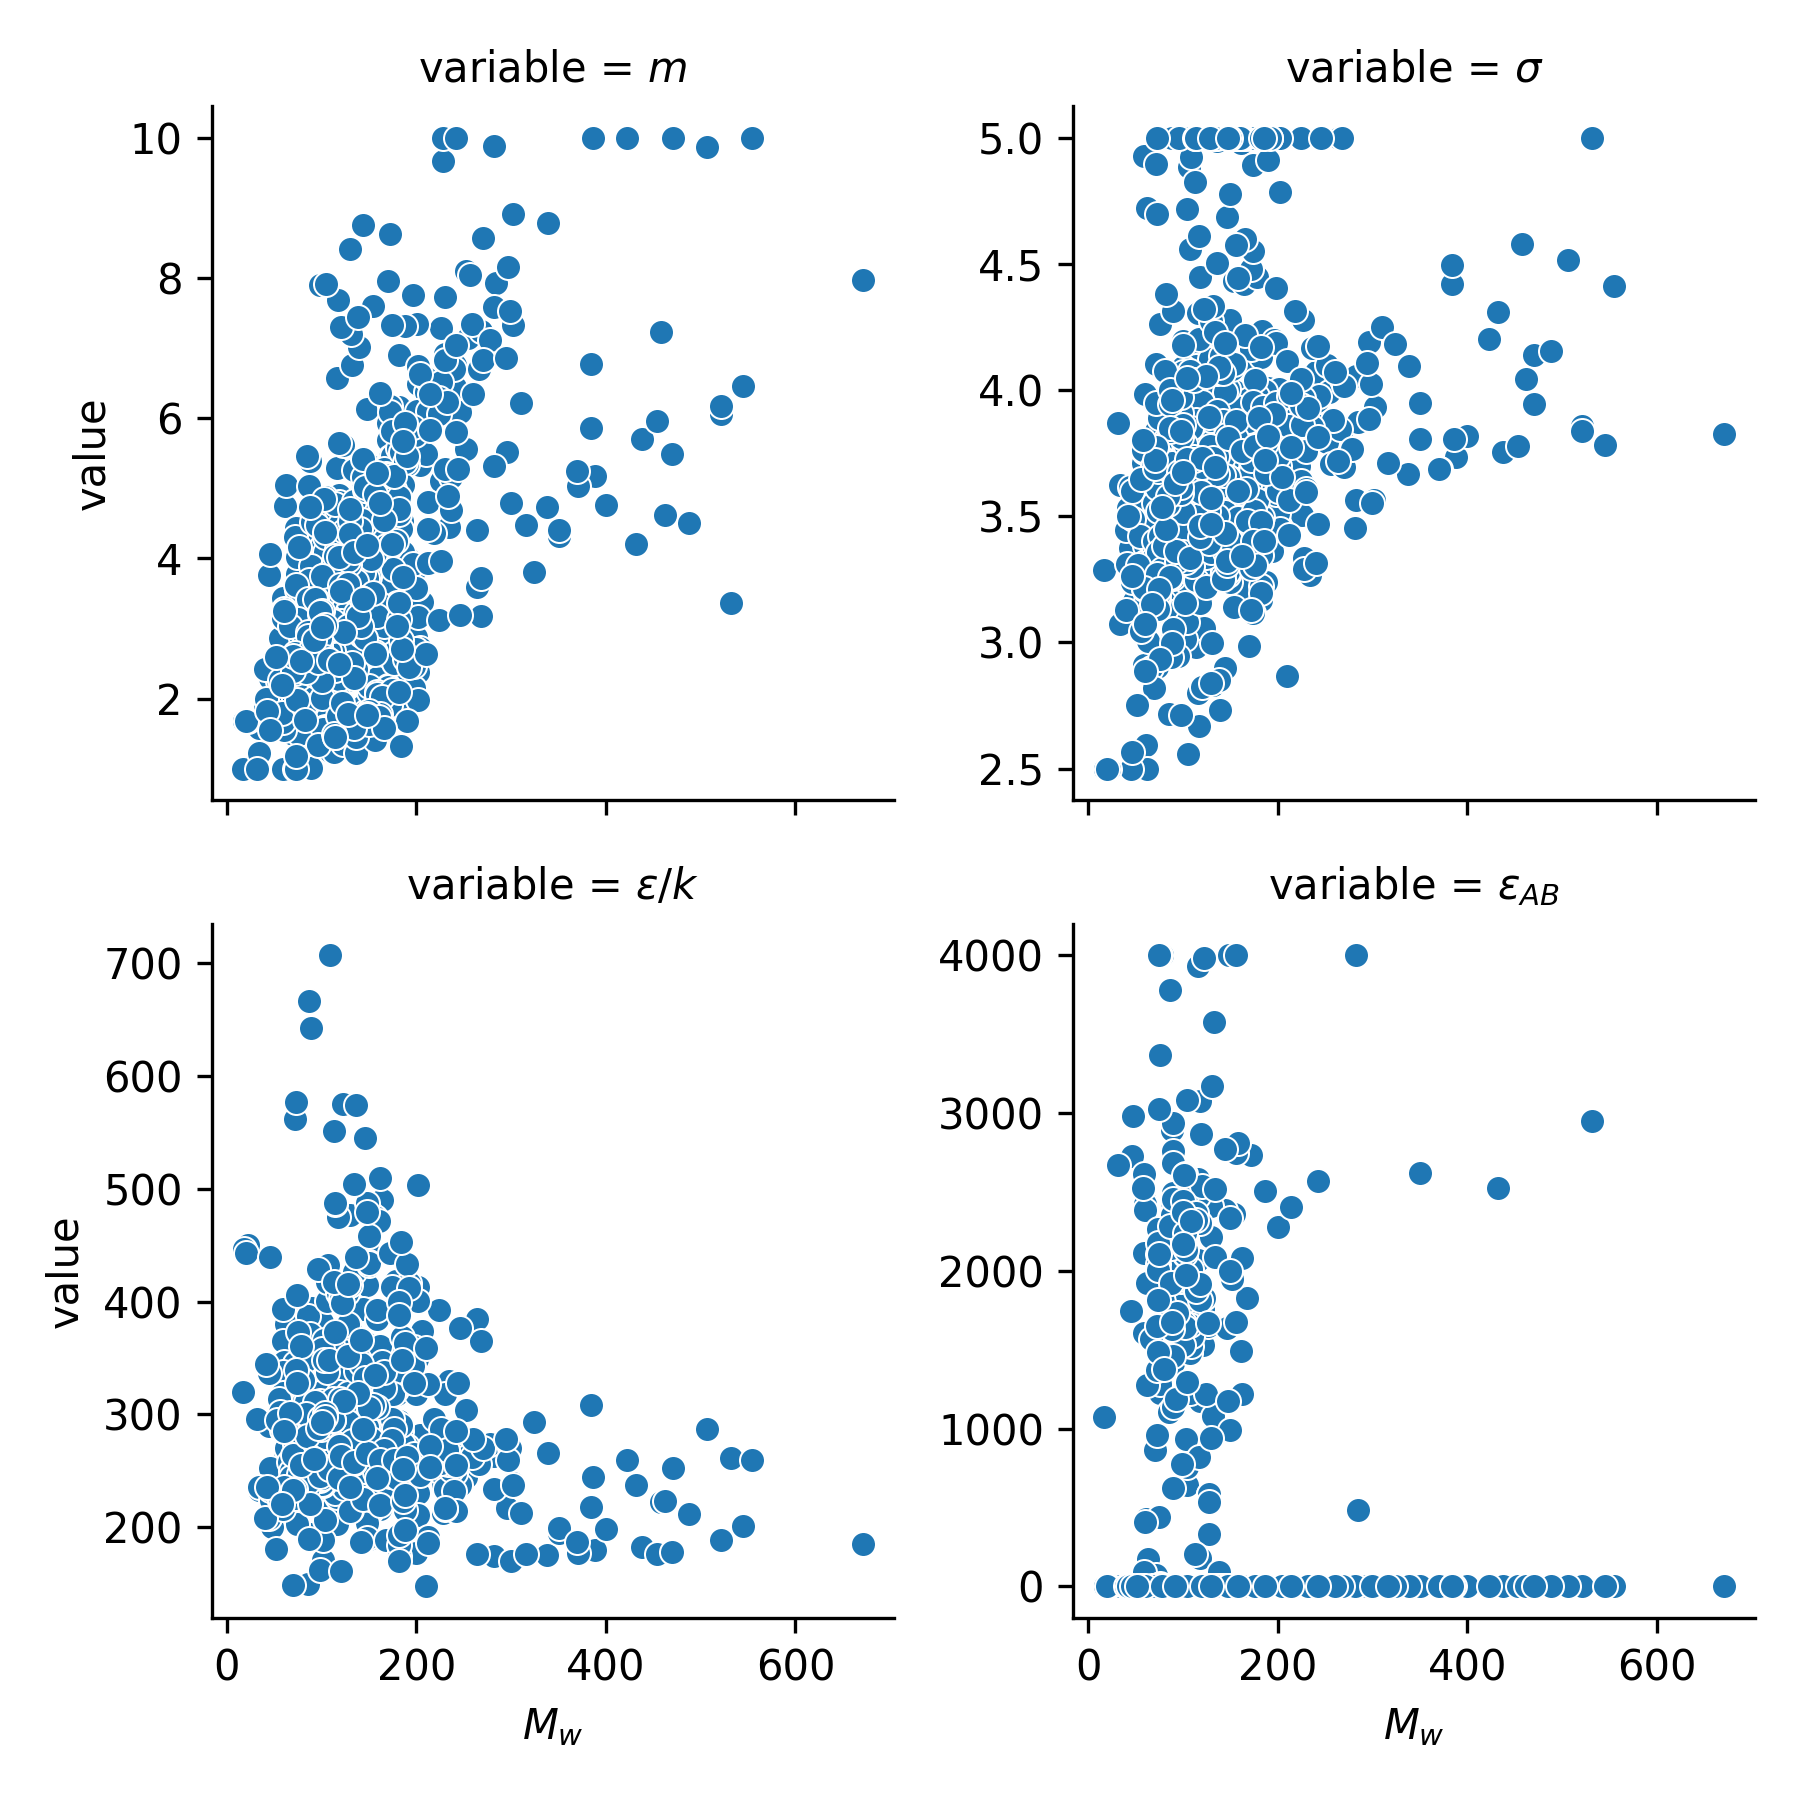
\includegraphics[width=0.8\textwidth]{gfx/Chapter07/mw_pcsaft_parameter_correlation.png}
    \caption{Correlation between molecular weight and PCP-SAFT parameters predicted by ML-SAFT.}
    \label{fig:molecular_weight}
\end{figure}

\section{Hyperparameter Tuning}

The hyperparameters for each model were explored using a quasi-random design \cite{Bosquet2017} with a budget of 100 trials. The hyperparameters tuned for each model are shown in Table \ref{tab:hyperparameters}. The best hyperparameters for each model architecture was selected by evaluating the sum of the RMSE for all PCP-SAFT parameters.

\begin{table}
	\caption{Hyperparameters tuned for each model and their final values after 100 quasi-random trials.}
        \tiny
	\begin{center}
		\begin{tabular}{lp{.2\textwidth}p{.4\textwidth}l}
			Pipeline & Hyperparameter & Configuration & Final value \\
			\hline
			FFN & Fp Bits & 1024, 4096, 16384 & 1024 \\
			 & Num Hidden Layers & 1, 2, 3, 4, 5, 6 & 2 \\
			 & Target Columns & ['m', 'sigma', 'epsilon k', 'epsilonAB'],\par['m', 'sigma', 'epsilon k', 'epsilonAB', 'KAB'],\par['m', 'sigma', 'epsilon k', 'epsilonAB', 'mu'] & m,sigma,epsilon k,epsilonAB,mu \\
			 & Balanced Associating Sampling & True, False & False \\
			 & Filter Non Associating Inside Loss & True, False & True \\
			 & Dropout & 0.0 - 0.5 & 0.18 \\
			 & LR & 1e-05 - 0.1 & 6.51e-03 \\
			 & Optimizer & adam & adam \\
			 & Beta 1 & 0.8 - 0.99 & 8.56e-01 \\
			 & Scheduler & noam & noam \\
			 & Warmup Epochs & 1 - 10 & 5 \\
			 & Max Lr Ratio & 2 - 100 & 24.36 \\
			 & Final Lr Ratio & 0.1 - 1.0 & 0.30 \\
			D-MPNN & Num Convs & 1, 2, 3 & 1 \\
			 & Dim Fingerprint & 32 - 350 & 109 \\
			 & Pool Type & mean, add & mean \\
			 & Target Columns & ['m', 'sigma', 'epsilon k', 'epsilonAB'],\par['m', 'sigma', 'epsilon k', 'epsilonAB', 'KAB'],\par['m', 'sigma', 'epsilon k', 'epsilonAB', 'mu'] & m,sigma,epsilon k,epsilonAB \\
			 & Balanced Associating Sampling & True, False & True \\
			 & Filter Non Associating Inside Loss & True, False & True \\
			 & Dropout & 0.0 - 0.5 & 0.05 \\
			 & LR & 1e-05 - 0.1 & 3.50e-02 \\
			 & Optimizer & adam & adam \\
			 & Beta 1 & 0.8 - 0.99 & 8.97e-01 \\
			 & Scheduler & noam & noam \\
			 & Warmup Epochs & 1 - 10 & 3 \\
			 & Max Lr Ratio & 2 - 100 & 31.54 \\
			 & Final Lr Ratio & 0.1 - 1.0 & 0.55 \\
			MPNN & Num Convs & 1, 2, 3 & 1 \\
			 & Dim Fingerprint & 32 - 350 & 39 \\
			 & Pool Type & mean, add & add \\
			 & Target Columns & ['m', 'sigma', 'epsilon k', 'epsilonAB'],\par['m', 'sigma', 'epsilon k', 'epsilonAB', 'KAB'],\par['m', 'sigma', 'epsilon k', 'epsilonAB', 'mu'] & m,sigma,epsilon k,epsilonAB,mu \\
			 & Balanced Associating Sampling & True, False & True \\
			 & Filter Non Associating Inside Loss & True, False & False \\
			 & Dropout & 0.0 - 0.5 & 0.45 \\
			 & LR & 1e-05 - 0.1 & 8.06e-03 \\
			 & Optimizer & adam & adam \\
			 & Beta 1 & 0.8 - 0.99 & 9.48e-01 \\
			 & Scheduler & noam & noam \\
			 & Warmup Epochs & 1 - 10 & 1 \\
			 & Max Lr Ratio & 2 - 100 & 61.65 \\
			 & Final Lr Ratio & 0.1 - 1.0 & 0.35 \\
		\end{tabular}
	\end{center}
	\label{tab:hyperparameters}
\end{table}

As an example, Figure \ref{fig:ML-SAFT_sweep_parallel_plot} shows a visualization of a hyperparameter sweep for the MPNN. The best models used a small learning rate ($<6\text{X}  10^{-5}$), and the overall effect of filtering non-associating molecules inside the loss function (verses as post-processing step) was negative.

\begin{figure}
    \centering
    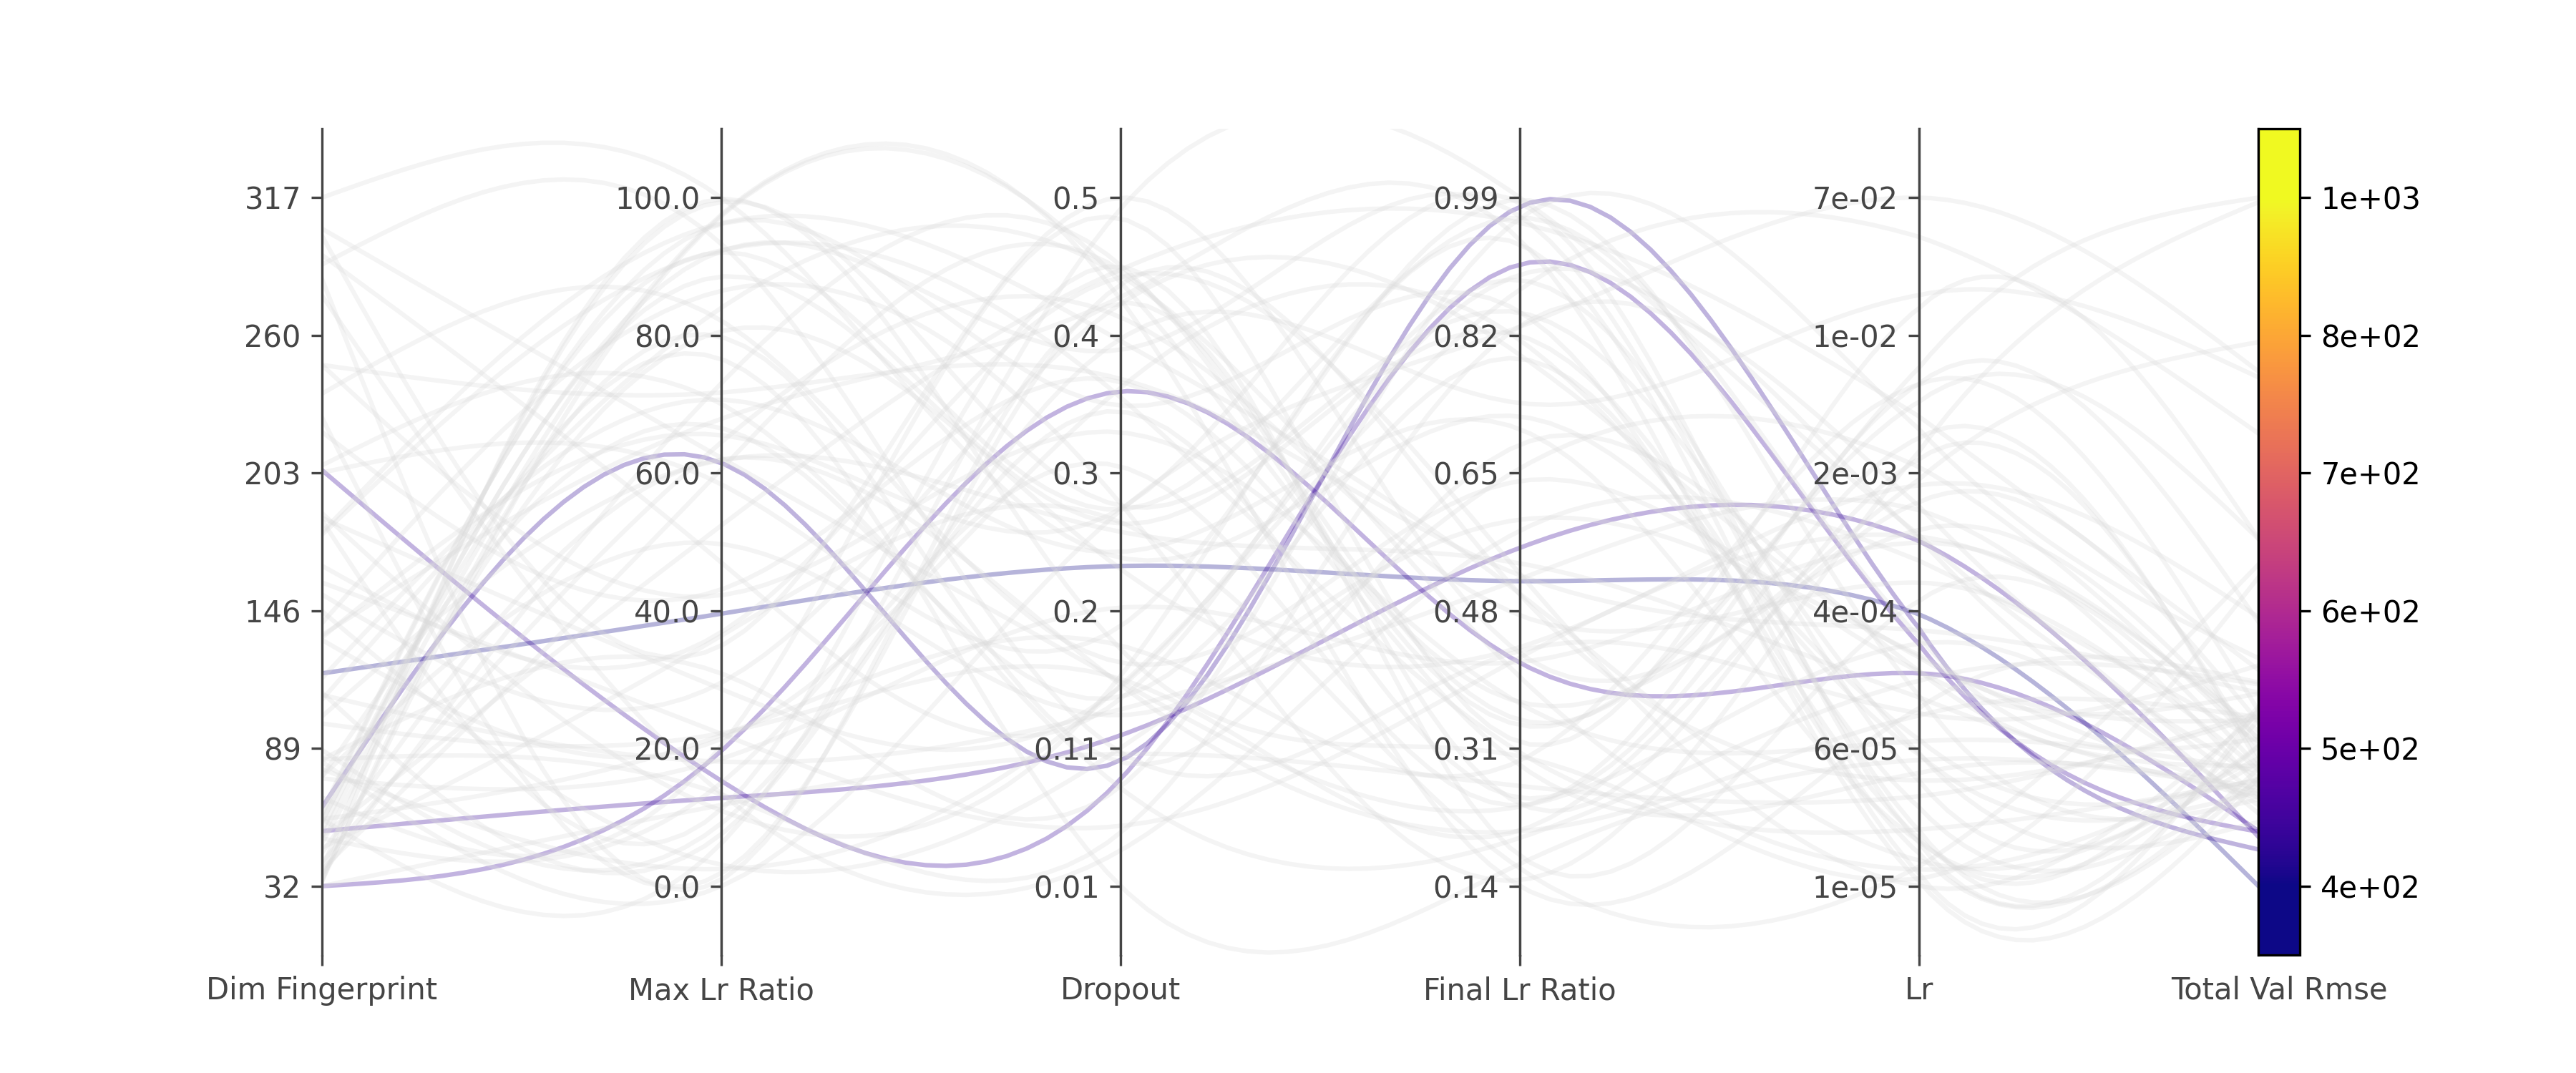
\includegraphics[width=\textwidth]{gfx/Chapter07/pyg_sweep_u157us_parallel_plot_total_val_rmse.png}
    \caption{Parallel plot showing the results of a hyperparameter sweep of ML-SAFT. The top five most important features are shown as determined by a RF fitted to predict the validation RMSE given the hyperparaemters. Furthermore, the runs with the five lowest total RMSE scores (i.e., summing all RMSE for all PC-SAFT parameter predictions) are highlighted.}
    \label{fig:ML-SAFT_sweep_parallel_plot}
\end{figure}

\section{Parity plots}\label{app:parity}

\begin{figure}
    \centering
    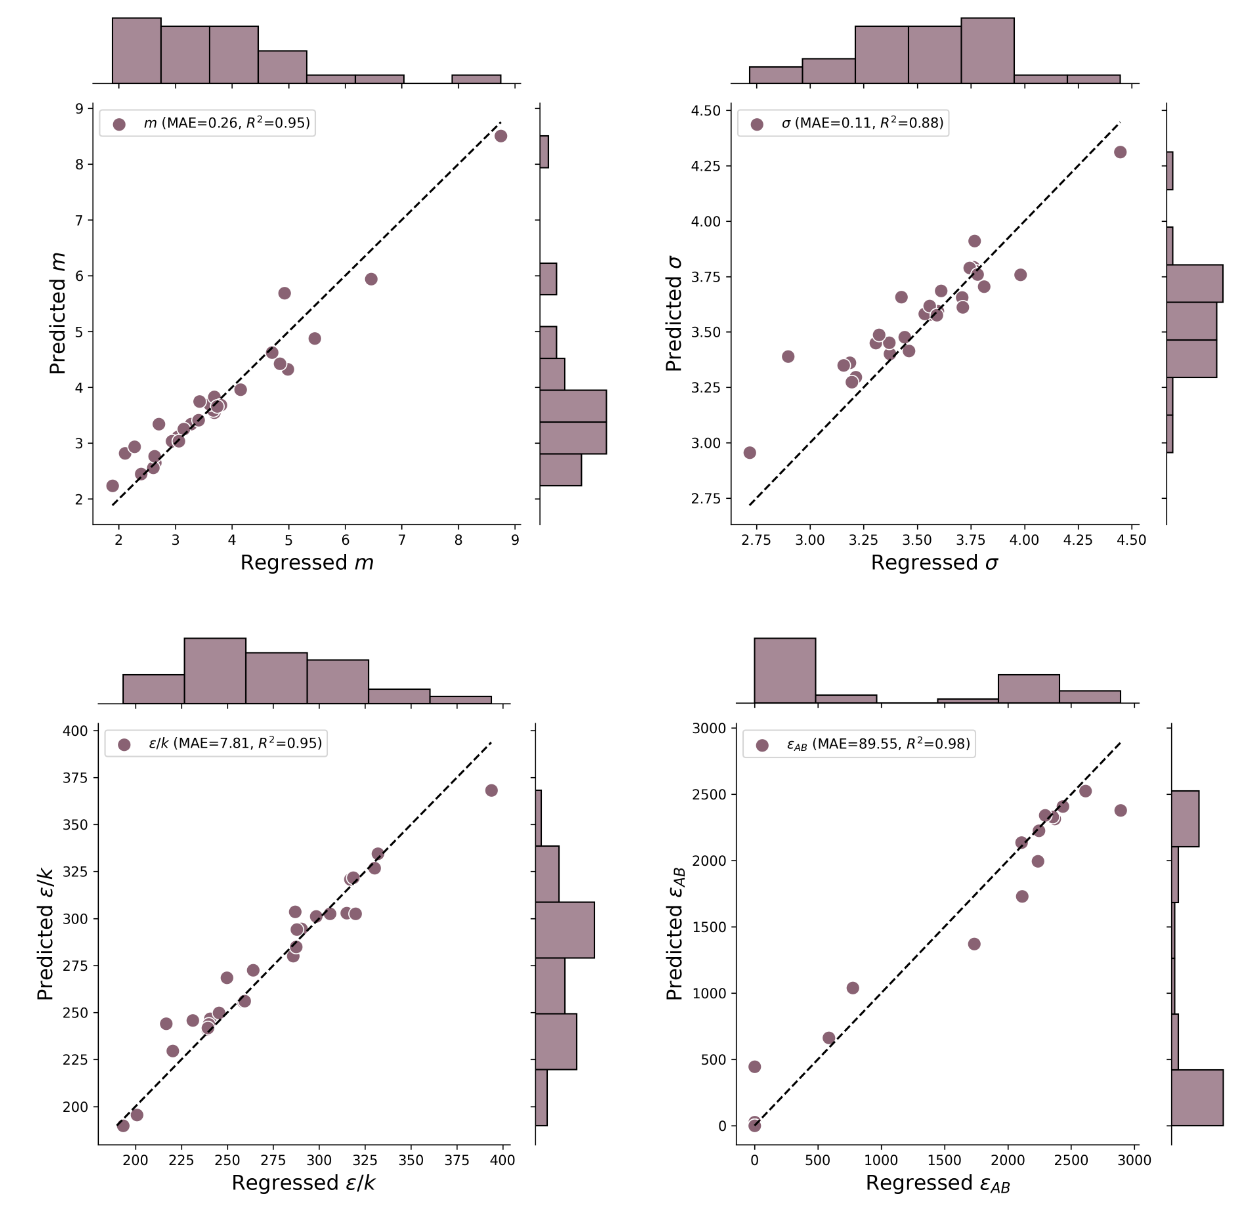
\includegraphics[width=\textwidth]{gfx/Chapter07/rf_parity_plots.png}
    \caption{Parity plots on the test dataset of predictions PCP-SAFT parameters using the random forest.}
    \label{fig:rf}
\end{figure}


\begin{figure}
    \centering
    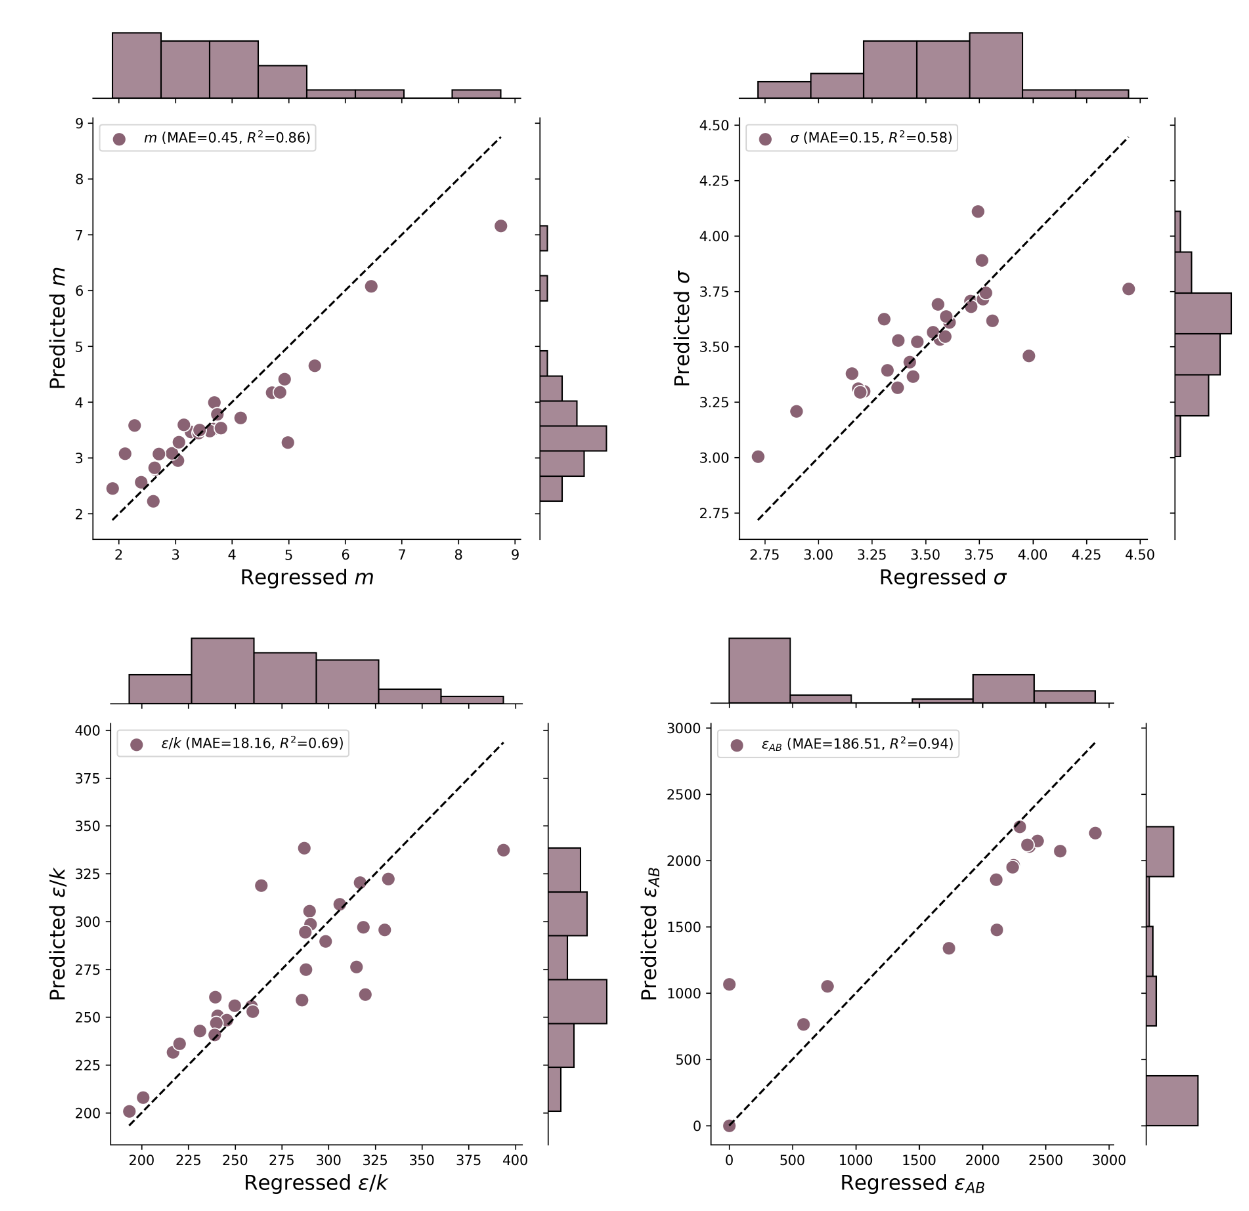
\includegraphics[width=\textwidth]{gfx/Chapter07/mpnn_parity_plots.png}
    \caption{Parity plots on the test dataset of predictions PCP-SAFT parameters using the MPNN.}
    \label{fig:mpnn}
\end{figure}


\begin{figure}
    \centering
    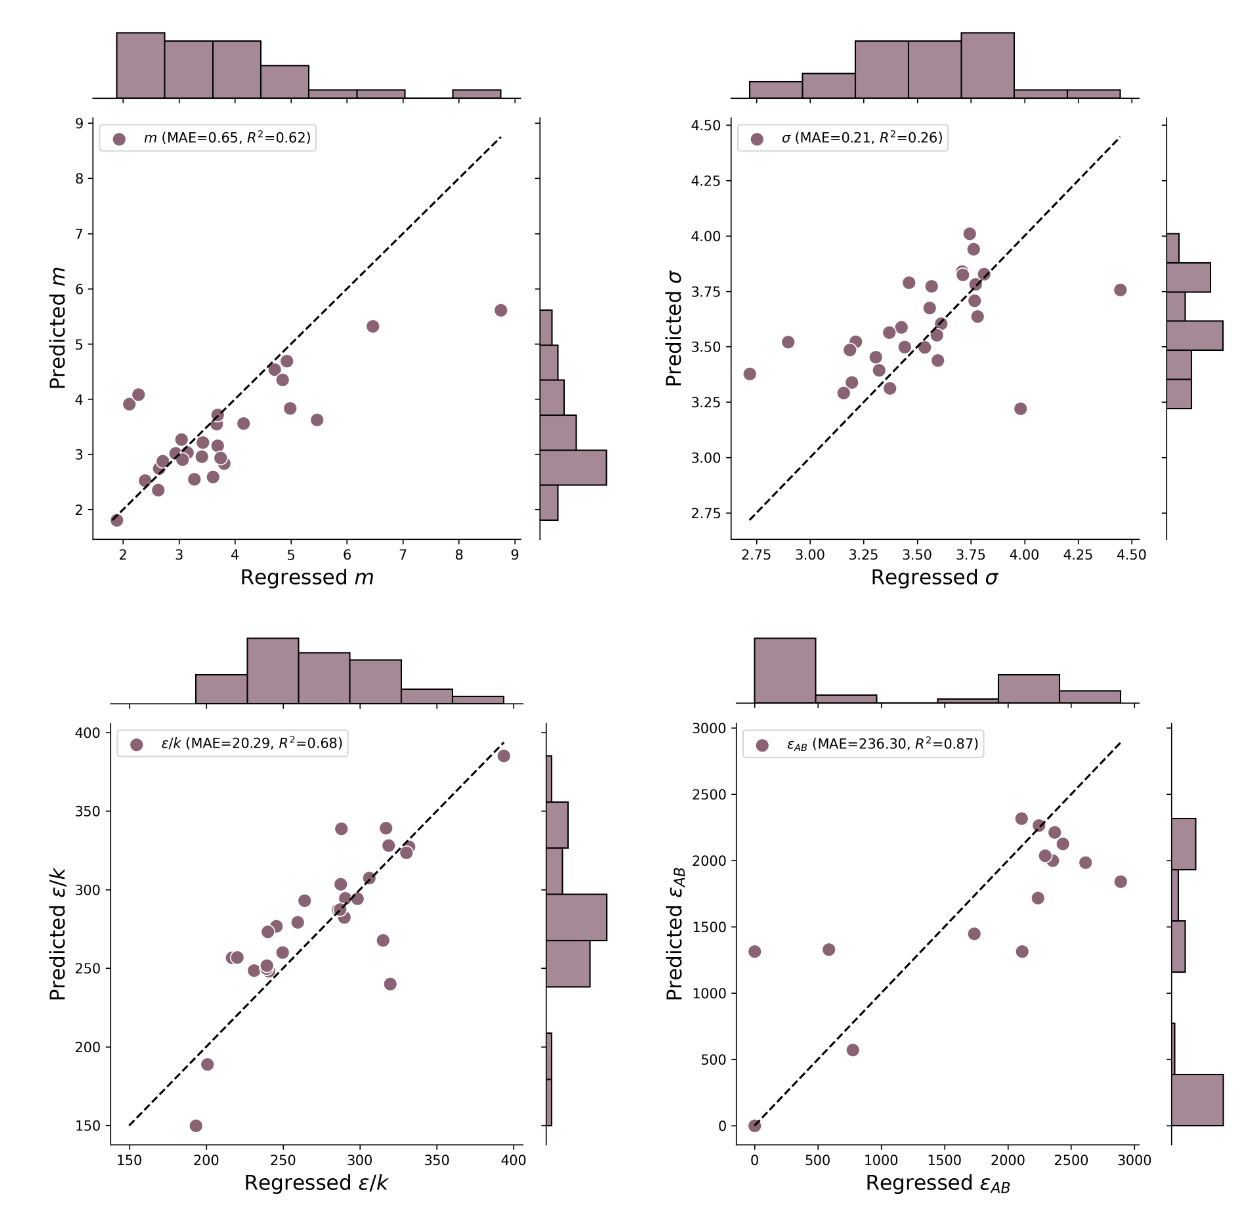
\includegraphics[width=\textwidth]{gfx/Chapter07/dmpnn_parity_plots.png}
    \caption{Parity plots on the test dataset of predictions PCP-SAFT parameters using the D-MPNN.}
    \label{fig:dmpnn}
\end{figure}

\begin{figure}
    \centering
    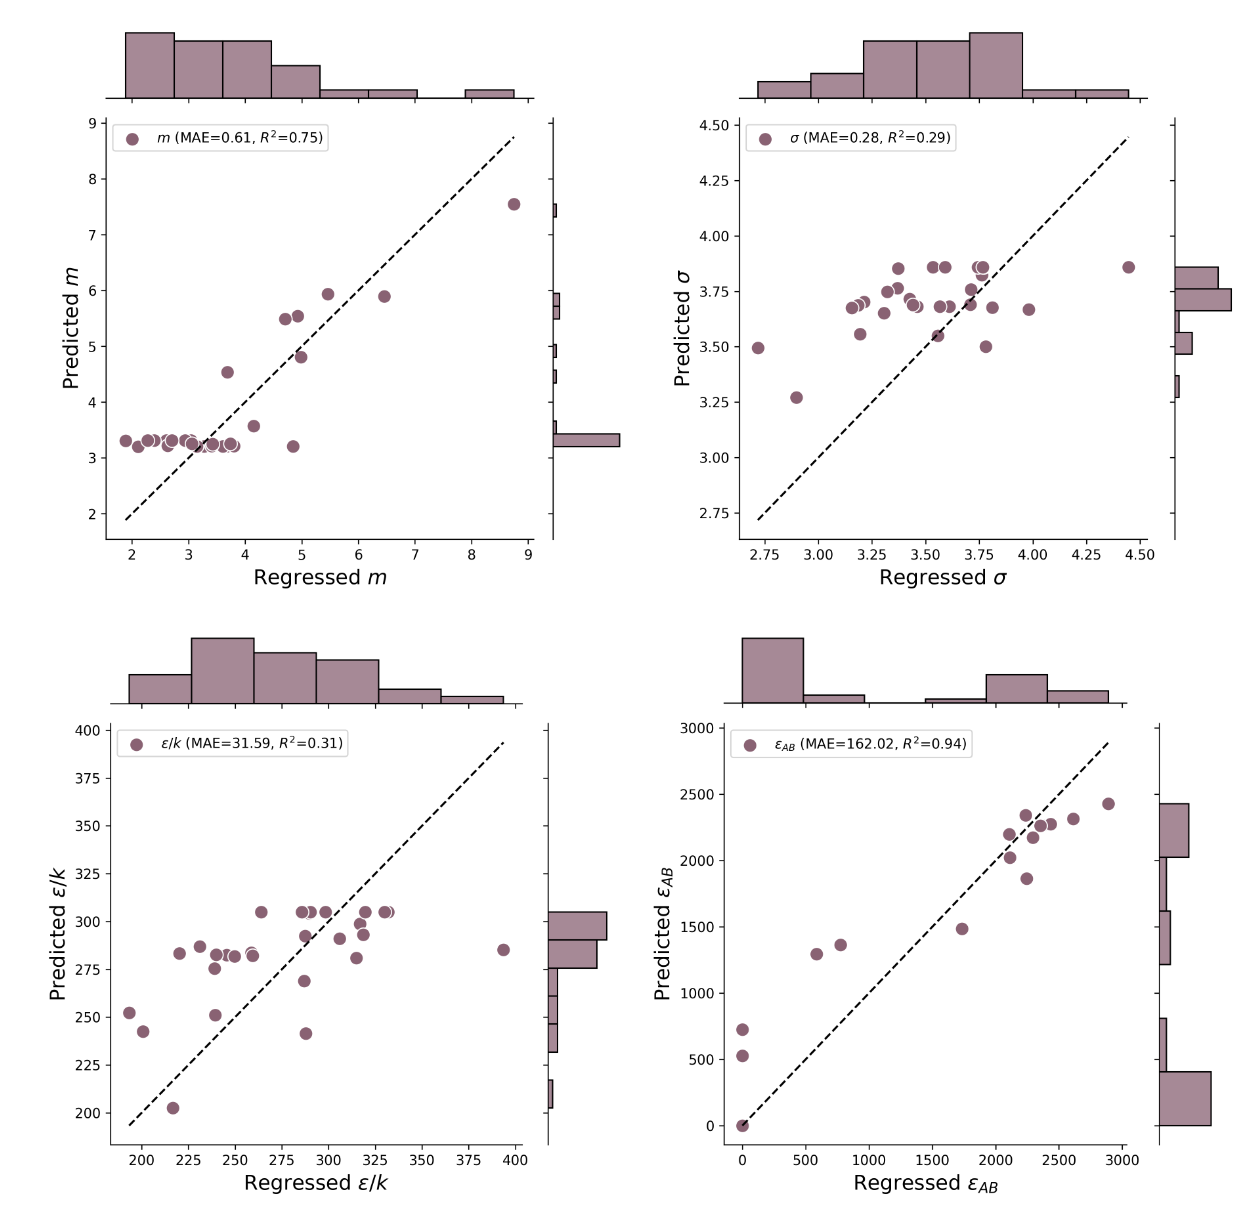
\includegraphics[width=\textwidth]{gfx/Chapter07/ffn_parity_plots.png}
    \caption{Parity plots on the test dataset of predictions PCP-SAFT parameters using the FFN.}
    \label{fig:ffn}
\end{figure}